\documentclass[conference]{IEEEtran}
\usepackage[utf8]{inputenc}
\usepackage[T1]{fontenc}
\usepackage{lmodern}
\usepackage{amsmath,amssymb}
\usepackage{graphicx}
\usepackage{booktabs}
\usepackage{array}
\usepackage{xcolor}
\usepackage{algorithm}
\usepackage{algpseudocode}
\usepackage{url}
\usepackage[hidelinks]{hyperref}
\usepackage{cite}
\graphicspath{{figures/v4/}{../results/ablation/figures/}}
\newcommand{\brierFull}{0.127}
\newcommand{\calFull}{1.37}
\newcommand{\calIsoAUC}{0.900}
\newcommand{\calIsoBrier}{0.127}
\newcommand{\calIsoSlope}{0.56}
\newcommand{\calOnehotAUC}{0.903}
\newcommand{\calOnehotBrier}{0.127}
\newcommand{\calOnehotSlope}{1.39}
\newcommand{\calPlattAUC}{0.900}
\newcommand{\calPlattBrier}{0.125}
\newcommand{\calPlattSlope}{1.13}
\newcommand{\clinAUC}{0.906}
\newcommand{\clinAUCci}{[0.864, 0.947]}
\newcommand{\clinAcc}{0.826}
\newcommand{\clinLRAUCval}{0.904}
\newcommand{\concatAUC}{0.878}
\newcommand{\dClinAUC}{+0.004 [-0.009, +0.017]}
\newcommand{\dClinAcc}{+0.3 [-2.2, +2.7]}
\newcommand{\dClinLRAUC}{+0.003 [-0.017, +0.022]}
\newcommand{\dConcat}{-0.009 [-0.030, +0.012]}
\newcommand{\dGbmOnlyAUC}{-0.018 [-0.034, -0.002]}
\newcommand{\dHardAUC}{-0.032 [-0.053, -0.011]}
\newcommand{\dLRAUC}{-0.004 [-0.025, +0.017]}
\newcommand{\dNoSmoteAUC}{-0.002 [-0.009, +0.006]}
\newcommand{\dNoSmoteAcc}{+1.1 [-0.6, +2.7]}
\newcommand{\dProxyOnlyAUC}{-0.089 [-0.132, -0.046]}
\newcommand{\dRfOnlyAUC}{-0.022 [-0.041, -0.002]}
\newcommand{\dStackAUC}{-0.000 [-0.005, +0.005]}
\newcommand{\dSvmOnlyAUC}{+0.004 [-0.015, +0.023]}
\newcommand{\dTokens}{+0.006 [-0.023, +0.036]}
\newcommand{\dXgbOnlyAUC}{-0.007 [-0.020, +0.006]}
\newcommand{\defaultXgbAUC}{0.875}
\newcommand{\dupShareMean}{22\%}
\newcommand{\ecgCleanAUC}{0.845}
\newcommand{\ecgLeadIAUC}{0.724}
\newcommand{\ecgMinIIAUC}{0.666}
\newcommand{\ecgNoisyAUC}{0.780}
\newcommand{\ecgNoisyN}{72}
\newcommand{\ecgRefAUC}{0.819}
\newcommand{\ecgSizeList}{n=303: 0.823; n=606: 0.800; n=1212: 0.825}
\newcommand{\ecgTwelveMinAUC}{0.768}
\newcommand{\ecgTwelvePlusAUC}{0.823}
\newcommand{\ecgVFiveAUC}{0.819}
\newcommand{\ecgVOneAUC}{0.752}
\newcommand{\engMaxAbs}{0.004}
\newcommand{\extDeltaList}{Hungary: +0.004 [-0.007, +0.015]; Switzerland: -0.013 [-0.069, +0.035]; VA Long Beach: -0.013 [-0.035, +0.008]}
\newcommand{\extHunCl}{0.886}
\newcommand{\extHunFu}{0.889}
\newcommand{\extSwiCl}{0.785}
\newcommand{\extSwiFu}{0.772}
\newcommand{\extVaCl}{0.721}
\newcommand{\extVaFu}{0.709}
\newcommand{\fixedXgbAUC}{0.895}
\newcommand{\fullAUC}{0.902}
\newcommand{\fullAUCci}{[0.858, 0.945]}
\newcommand{\fullAcc}{0.823}
\newcommand{\fullSens}{0.773}
\newcommand{\fullSpec}{0.867}
\newcommand{\gbmOnlyAUCval}{0.884}
\newcommand{\hardAUCval}{0.869}
\newcommand{\hoClAcc}{0.831 (2.5--97.5\%: 0.738--0.902)}
\newcommand{\hoClAccPct}{81}
\newcommand{\hoClAccSeed}{0.869}
\newcommand{\hoDAUC}{-0.007 (2.5--97.5\%: -0.034--0.017)}
\newcommand{\hoDAUCPct}{94}
\newcommand{\hoDAUCSeed}{0.012}
\newcommand{\hoDAcc}{0.002 (2.5--97.5\%: -0.049--0.049)}
\newcommand{\hoDAccPct}{90}
\newcommand{\hoDAccSeed}{0.033}
\newcommand{\hoFuAUC}{0.904 (2.5--97.5\%: 0.832--0.955)}
\newcommand{\hoFuAUCPct}{99}
\newcommand{\hoFuAUCSeed}{0.96}
\newcommand{\hoFuAcc}{0.833 (2.5--97.5\%: 0.754--0.918)}
\newcommand{\hoFuAccPct}{95}
\newcommand{\hoFuAccSeed}{0.902}
\newcommand{\hoN}{200}
\newcommand{\lRAUCval}{0.898}
\newcommand{\leakPreAUC}{0.902}
\newcommand{\leakSmoteAUC}{0.916}
\newcommand{\linearAUC}{0.885}
\newcommand{\mlpClinAUC}{0.892}
\newcommand{\nVariants}{94}
\newcommand{\nestedAUC}{0.900}
\newcommand{\noSmoteAUCval}{0.900}
\newcommand{\noSmoteSens}{0.763}
\newcommand{\noSmoteSpec}{0.895}
\newcommand{\noiseAUC}{0.899}
\newcommand{\nonecgAUC}{0.903}
\newcommand{\pClinLR}{1.000}
\newcommand{\pGbmOnly}{0.558}
\newcommand{\pHard}{0.067}
\newcommand{\pLR}{1.000}
\newcommand{\pNoSmote}{1.000}
\newcommand{\pProxyOnly}{0.003}
\newcommand{\pRfOnly}{0.510}
\newcommand{\pStack}{1.000}
\newcommand{\pSvmOnly}{1.000}
\newcommand{\pXgbOnly}{1.000}
\newcommand{\permN}{100}
\newcommand{\permNull}{0.497}
\newcommand{\permNullSd}{0.049}
\newcommand{\permObs}{0.907}
\newcommand{\permP}{0.010}
\newcommand{\proxyOnlyAUCval}{0.813}
\newcommand{\rfOnlyAUCval}{0.880}
\newcommand{\robMaxD}{+0.004}
\newcommand{\robMinD}{-0.014}
\newcommand{\robN}{17}
\newcommand{\robNoAngioCl}{0.866}
\newcommand{\robNoAngioD}{-0.002 [-0.015, +0.012]}
\newcommand{\robNoAngioFu}{0.864}
\newcommand{\robNoExCl}{0.901}
\newcommand{\robNoExD}{+0.004 [-0.003, +0.012]}
\newcommand{\robNoExFu}{0.905}
\newcommand{\robNoiseCl}{0.877}
\newcommand{\robNoiseD}{-0.014 [-0.033, +0.005]}
\newcommand{\robNoiseFu}{0.863}
\newcommand{\robNsig}{0}
\newcommand{\robRestCl}{0.834}
\newcommand{\robRestD}{+0.003 [-0.009, +0.015]}
\newcommand{\robRestFu}{0.837}
\newcommand{\robSmallCl}{0.882}
\newcommand{\robSmallD}{-0.010 [-0.029, +0.008]}
\newcommand{\robSmallFu}{0.872}
\newcommand{\shapJac}{0.74}
\newcommand{\shapRhoFold}{0.90}
\newcommand{\shapRhoPI}{0.27}
\newcommand{\shapRhoSeed}{0.95}
\newcommand{\shuffledAUC}{0.897}
\newcommand{\smoteDupGap}{0.0\%}
\newcommand{\smoteInconsistent}{13.6\%}
\newcommand{\smoteNonInt}{100.0\%}
\newcommand{\stackAUCval}{0.902}
\newcommand{\svmOnlyAUCval}{0.905}
\newcommand{\tokensAUC}{0.893}
\newcommand{\xattnAUC}{0.887}
\newcommand{\xgbOnlyAUCval}{0.895}

\newcommand{\revnote}[1]{#1}

\begin{document}

\title{MultiCardioFusion: An Explainable ECG-Proxy-Enhanced Clinical Prediction Framework for Heart Disease Classification, with a Controlled Ablation Study}

\author{\IEEEauthorblockN{Dhanvanth Yugandhar Raj}
\IEEEauthorblockA{Department of Computer Science, VIT University\\Biomedical AI Research Group}}

\maketitle

\begin{abstract}
Cardiovascular disease is the leading cause of death worldwide, and most machine-learning work on cardiac screening uses a single data source. MultiCardioFusion enriches the 13 clinical variables of the UCI Cleveland Heart Disease dataset with 23 ECG-proxy features derived from the same patients' resting-ECG and exercise-test measurements, benchmarks a parallel PTB-XL ECG branch with 568 tsfresh descriptors, and explains predictions with SHAP. Because Cleveland and PTB-XL contain different patients, the work is framed as ECG-proxy-enhanced clinical prediction, not patient-level multimodal fusion. An earlier version reported AUC 0.9535 and a 7.04-point accuracy gain from fusion on a single 61-patient hold-out. Here every claim is re-tested under a controlled protocol: all preprocessing inside training folds, 5$\times$10 repeated cross-validation with identical splits and tuning budget, corrected confidence intervals and Holm-adjusted tests, over \nVariants{} configurations. These include component removal, negative controls, a permutation test, eight imbalance strategies, leakage and hold-out sensitivity analyses, 16 robustness scenarios, subgroups, external validation on three hospitals, SHAP stability, cross-attention variants and a PTB-XL lead and feature ablation. The full system reaches AUC \fullAUC{} \fullAUCci{}, but the clinical variables alone perform equally ($\Delta$AUC \dClinAUC{} in favour of clinical-only). The proxy block performs no better than added noise. The reported gain arose from subtracting a cross-validation accuracy from a hold-out accuracy of a different model, on a split that lies at the 95th percentile of \hoN{} random splits. SMOTE and length-1 cross-attention add nothing, oversampling before cross-validation inflates AUC, and external AUC ranges from \extVaFu{} to \extHunFu{}. SHAP rankings of \texttt{cp}, \texttt{ca} and \texttt{thal} are stable, while credit given to engineered features is redistributed from their parent variables. Because the dominant predictors come from fluoroscopy and thallium scintigraphy, the model is a post-test classifier and is not validated for clinical use. The study provides a leakage-aware, fully ablated baseline and shows how evaluation choices can create apparent fusion gains on small clinical datasets.
\end{abstract}

\begin{IEEEkeywords}
heart disease prediction, ablation study, ECG-proxy features, repeated cross-validation, data leakage, SHAP stability, external validation, calibration, tsfresh, PTB-XL.
\end{IEEEkeywords}

\section{Introduction}
Heart disease remains the leading cause of death worldwide~\cite{who2023}, which motivates automated tools for early detection. In practice, cardiologists combine several sources of evidence (blood tests, patient history, imaging and the electrocardiogram) before reaching a diagnosis. Most published machine-learning models for heart-disease prediction, however, use a single data source and therefore lack part of the clinical context that a diagnosis relies on.

The field has developed along two largely separate lines. Structured tabular datasets such as the UCI Cleveland Heart Disease dataset have been the standard testbed for clinical-feature-based classification since Detrano \emph{et al.}~\cite{detrano1989}, with reported accuracies rising from 77\% for early logistic regression to over 93\% for ensemble and neural models~\cite{arabasadi2017,haq2018,mohan2019}. In parallel, large waveform datasets such as PTB-XL, with 21{,}837 ten-second 12-lead ECG recordings annotated by cardiologists~\cite{wagner2020}, have become the reference benchmark for ECG-based diagnosis. Pipelines that exploit both kinds of information while remaining interpretable are much less explored.

\textbf{Three kinds of ``clinical + ECG'' studies.} Because the term \emph{multimodal} is used loosely in this literature, we distinguish three categories~\cite{huang2020fusion}:
(i)~\emph{true patient-level multimodal fusion}, where clinical variables and ECG signals are recorded from the same patient at the same encounter;
(ii)~\emph{proxy-feature fusion}, where ECG information is approximated by features derived from ECG-related variables already present in the clinical table; and
(iii)~\emph{parallel ECG benchmarking}, where an ECG-only model is trained and evaluated on a separate cohort with its own labels.
Cleveland and PTB-XL were collected at different institutions, in different decades, from different patients, so no Cleveland patient has a PTB-XL recording. This work therefore belongs to categories (ii) and (iii) and makes \emph{no claim of true patient-level fusion}.

This manuscript is a revision of an earlier version (v4) that reported AUC $=0.9535$ and a $+7.04$ percentage-point accuracy gain from fusion. Those figures came from a single 61-patient hold-out split, with preprocessing fitted on all patients and no confidence intervals, and the gain compared a hold-out score with a cross-validation score. Following reviewer feedback, the central aim of this revision is to \emph{test} each claim under a controlled protocol rather than to report a single best number. We address four research questions:
\begin{itemize}
\item \textbf{RQ1:} Do ECG-proxy features improve discrimination over the 13 clinical variables alone?
\item \textbf{RQ2:} Which pipeline components (feature groups, resampling, ensemble, cross-attention) contribute measurably?
\item \textbf{RQ3:} How robust are the conclusions to leakage, the evaluation protocol, data perturbations and a change of hospital?
\item \textbf{RQ4:} Are the SHAP explanations stable enough to support clinical interpretation?
\end{itemize}

The contributions of this work are:
\begin{itemize}
\item A \emph{leakage-aware ECG-proxy pipeline} in which imputation, feature derivation, scaling and resampling are all fitted inside training folds only.
\item A \emph{controlled comparison} of clinical-only, ECG-proxy-only and proxy-enhanced models, and of feature fusion, soft and hard voting, stacking and dual-branch networks with and without cross-attention, all under identical splits and tuning budget.
\item An \emph{extended ablation study} of \nVariants{} configurations: component removal with corrected confidence intervals, negative controls and a permutation test, six imbalance strategies, leakage and hold-out sensitivity analyses, 16 robustness and edge-case scenarios, subgroup analyses, external validation on three further hospitals, and a PTB-XL ECG-branch ablation.
\item \emph{SHAP global and local interpretability} together with stability measurements across folds and seeds and agreement with permutation importance.
\item An explicit, quantified account of the \emph{limitation of non-paired datasets} and of which v4 claims do and do not survive.
\end{itemize}

Section~II reviews related work. Section~III describes the datasets and Section~IV the methodology and evaluation protocol. Section~V reports baseline and fusion results, and Section~VI the extended ablation study. Section~VII discusses interpretability, Section~VIII the findings against the research questions, and Section~IX concludes.

\section{Related Work and Baselines}
\subsection{Clinical Feature-Based Cardiac Prediction}
Prediction on the UCI Cleveland dataset has moved from the logistic probability algorithm of Detrano \emph{et al.}~\cite{detrano1989} (about 77\% accuracy) to machine-learning and ensemble methods. Examples are the hybrid random forest with a linear model (HRFLM) of Mohan \emph{et al.}~\cite{mohan2019} (88.7\% accuracy), the majority-voting ensemble of Latha and Jeeva~\cite{latha2019} (85.48\%), the feature-selection study of Haq \emph{et al.}~\cite{haq2018} (89\% with logistic regression on Relief-selected features, 10-fold CV), and bagged decision trees with PCA by Gao \emph{et al.}~\cite{gao2021} (98.6\%). Results on the different Z-Alizadeh Sani dataset (303 patients, 54 features), such as the 93.85\% of Arabasadi \emph{et al.}~\cite{arabasadi2017}, are sometimes quoted alongside Cleveland results but concern another cohort. A limitation shared by Cleveland studies is the small cohort ($N=303$): a 10-fold test fold holds about 30 patients, so accuracy estimates vary considerably between folds and their confidence intervals are wide. Reported accuracies near or above 95\% should therefore be compared with others only when the validation protocol, in particular whether feature extraction and resampling were fitted inside the folds, is known to be equivalent. Section~VI-D shows that one common protocol error, oversampling before cross-validation, inflates AUC on this dataset.

\subsection{ECG Signal Analysis}
PTB-XL~\cite{wagner2020} enabled systematic benchmarking of ECG classifiers. Hannun \emph{et al.}~\cite{hannun2019} achieved cardiologist-level classification of 12 rhythm classes from single-lead ambulatory ECGs with a 34-layer deep neural network trained on more than 90{,}000 recordings. Ribeiro \emph{et al.}~\cite{ribeiro2020} trained a deep residual network on about 2.3 million 12-lead ECGs and reported F1 scores above 80\% for six abnormalities, outperforming cardiology residents. These studies differ from ours in two important ways: they use far larger training sets, and they predict \emph{ECG diagnostic statements} or rhythms, not angiographically confirmed coronary artery disease. Their accuracy figures are therefore not comparable with Cleveland results.

\subsection{Multimodal and Cross-Modal Fusion}
Combining data types is a major direction in medical AI, and a systematic review of imaging--EHR fusion~\cite{huang2020fusion} describes early (feature-level), joint and late fusion strategies. A single modality can also carry information usually obtained elsewhere: Attia \emph{et al.}~\cite{attia2019} detected left-ventricular systolic dysfunction (ejection fraction $\leq$35\%) from the 12-lead ECG alone with AUC 0.93. Cross-attention~\cite{vaswani2017} is increasingly used to let one modality condition on another. \emph{True} multimodal fusion, however, requires that the modalities describe the same patient, visit or event~\cite{huang2020fusion}. When they do not, as with Cleveland and PTB-XL, a model can at best approximate one modality from the other (proxy fusion) or evaluate each modality separately (parallel benchmarking). MultiCardioFusion uses proxy-aligned fusion on Cleveland and parallel ECG benchmarking on PTB-XL (Section~I).

\subsection{Explainability in Clinical AI}
SHAP~\cite{lundberg2017} is widely used for clinical models on structured data, and TreeSHAP~\cite{lundberg2018tree} computes exact Shapley values for tree ensembles such as XGBoost efficiently. In clinical use, Lundberg \emph{et al.}~\cite{lundberg2018sepsis} showed anaesthesiologists real-time SHAP explanations of intra-operative hypoxaemia risk. Three caveats apply. First, SHAP values are \emph{post-hoc and associational}: they describe the model, not causal mechanisms in the patient~\cite{kumar2020problems}. Second, with small samples and correlated or duplicated features, attributions can be split arbitrarily between features and can change between training runs~\cite{molnar2022pitfalls}. Third, agreement with known risk factors is necessary but not sufficient evidence of validity, and attributions can be manipulated~\cite{slack2020fooling}. We therefore treat SHAP as a descriptive tool, quantify its stability (Section~VI-H), and propose clinician review as future validation.

\begin{table*}[!t]
\centering\scriptsize
\caption{Literature summary and positioning of this work. Reported results are quoted as published; datasets, validation protocols and metrics differ between studies, so the figures are not directly comparable.}
\label{tab:lit}
\setlength{\tabcolsep}{3pt}
\begin{adjustbox}{max width=\linewidth}
\begin{tabular}{p{2.6cm}p{2.4cm}p{3.2cm}p{3.2cm}p{5.2cm}}
\toprule
Study & Data & Technique & Reported result & Relation to this work\\
\midrule
Detrano \emph{et al.}~\cite{detrano1989} 1989 & Cleveland (303) + other sites & Logistic probability algorithm & Acc.\ $\approx$77\% & Origin of the dataset and of the CAD label.\\
Haq \emph{et al.}~\cite{haq2018} 2018 & Cleveland (303) & 7 classifiers, Relief/mRMR/LASSO selection & Acc.\ 89\% (LR + Relief, 10-fold CV) & Clinical features only; no uncertainty estimates.\\
Mohan \emph{et al.}~\cite{mohan2019} 2019 & Cleveland (303) & HRFLM (RF + linear model) & Acc.\ 88.7\% & Clinical features only.\\
Latha \& Jeeva~\cite{latha2019} 2019 & Cleveland (303) & Bagging, boosting, stacking, majority voting & Acc.\ 85.48\% (majority voting) & Clinical features only; no explanations.\\
Gao \emph{et al.}~\cite{gao2021} 2021 & Cleveland (303) & Bagging/boosting with PCA/LDA & Acc.\ 98.6\% & Comparability depends on protocol details (Section~VI-D).\\
Arabasadi \emph{et al.}~\cite{arabasadi2017} 2017 & Z-Alizadeh Sani (303, 54 features) & GA-initialised neural network & Acc.\ 93.85\% & Different dataset; listed because it is often compared with Cleveland.\\
Hannun \emph{et al.}~\cite{hannun2019} 2019 & Single-lead ambulatory ECG ($>$90k) & 34-layer deep network & Cardiologist-level F1 (rhythm) & Rhythm labels; no clinical variables.\\
Ribeiro \emph{et al.}~\cite{ribeiro2020} 2020 & 12-lead ECG (2.3M) & Deep residual network & F1 $>$80\%, 6 abnormalities & ECG diagnostic labels, not CAD.\\
Attia \emph{et al.}~\cite{attia2019} 2019 & 12-lead ECG & Convolutional network & AUC 0.93 (EF $\leq$35\%) & ECG-only; different task.\\
\midrule
\textbf{This work (v5)} & Cleveland + 3 external sites; PTB-XL (parallel) & Proxy-enhanced clinical features; soft voting; dual-branch DL; SHAP & AUC \fullAUC{} \fullAUCci{} (5$\times$10 CV); clinical-only \clinAUC{} & Proxy fusion and parallel ECG benchmarking (not paired fusion); full ablation with CIs, controls and external validation.\\
\bottomrule
\end{tabular}
\end{adjustbox}
\end{table*}

\section{Datasets and Preprocessing}
\subsection{UCI Cleveland Heart Disease Dataset}
The Cleveland dataset (UCI repository, ID 45~\cite{janosi1989}) contains 303 patients referred for coronary angiography, each with 13 clinical variables (Table~\ref{tab:features}). The original target \texttt{num} (0--4) records angiographic disease status: 0 means $<$50\% diameter narrowing in every major vessel, and values 1--4 mean $>$50\% narrowing in at least one vessel~\cite{detrano1989}. Following common practice we binarise it as $y=1$ if \texttt{num}$>0$ (coronary artery disease, CAD) and $y=0$ otherwise. This gives \textbf{164 patients without CAD (54.1\%) and 139 with CAD (45.9\%)}. (The v4 manuscript paired these percentages with the wrong classes.) Table~\ref{tab:demo} summarises the cohort by class.

Two categorical variables have missing values: \texttt{ca} ($n=4$) and \texttt{thal} ($n=2$). Median imputation is used because the mean of a categorical code is not a valid category; rows are not dropped given the small cohort. \revnote{In this revision, the imputer, the feature derivation and the StandardScaler are fitted \emph{inside each training fold only} (Section~IV-G); in v4 they were fitted on all 303 patients before splitting.}

The variables \texttt{cp}, \texttt{restecg}, \texttt{slope} and \texttt{thal} are categorical codes. Standardising them as if they were continuous assumes equally spaced, ordered categories. This is harmless for tree models, which split on thresholds, but not for SVM or logistic regression. We therefore compare ordinal coding with one-hot coding in Section~VI-F.

\begin{table}[!t]
\centering\scriptsize
\caption{Cleveland Heart Disease dataset features.}
\label{tab:features}
\begin{adjustbox}{max width=\linewidth}
\begin{tabular}{lll}
\toprule
Feature & Description & Type\\
\midrule
age & Age in years & Continuous\\
sex & Sex (1 = male, 0 = female) & Binary\\
cp & Chest-pain type (1--4; 4 = asymptomatic) & Categorical\\
trestbps & Resting blood pressure (mm Hg) & Continuous\\
chol & Serum cholesterol (mg/dL) & Continuous\\
fbs & Fasting blood sugar $>$ 120 mg/dL & Binary\\
restecg & Resting ECG (0 normal, 1 ST-T abnormality, 2 LVH) & Categorical\\
thalach & Maximum heart rate achieved & Continuous\\
exang & Exercise-induced angina & Binary\\
oldpeak & ST depression, exercise vs.\ rest & Continuous\\
slope & Peak-exercise ST slope (1 up, 2 flat, 3 down) & Ordinal\\
ca & Major vessels coloured by fluoroscopy (0--3) & Ordinal\\
thal & Thallium scan (3 normal, 6 fixed, 7 reversible defect) & Categorical\\
\bottomrule
\end{tabular}
\end{adjustbox}
\end{table}

\begin{table}[!t]
\centering
\scriptsize
\caption{Cleveland cohort by class (mean $\pm$ SD or n (\%); Mann--Whitney U or $\chi^2$ test).}
\label{tab:demo}
\setlength{\tabcolsep}{3pt}
\begin{adjustbox}{max width=\linewidth}
\begin{tabular}{lccc}
\toprule
Characteristic & No CAD & CAD & $p$ \\
\midrule
Patients, n & 164 & 139 & -- \\
Age, years & 52.6 $\pm$ 9.5 & 56.6 $\pm$ 7.9 & $<$0.001 \\
Female, n (\%) & 72 (44\%) & 25 (18\%) & $<$0.001 \\
Asymptomatic chest pain & 39 (24\%) & 105 (76\%) & $<$0.001 \\
Resting BP, mm Hg & 129.2 $\pm$ 16.2 & 134.6 $\pm$ 18.8 & 0.026 \\
Cholesterol, mg/dL & 242.6 $\pm$ 53.5 & 251.5 $\pm$ 49.5 & 0.035 \\
Max.\ heart rate & 158.4 $\pm$ 19.2 & 139.3 $\pm$ 22.6 & $<$0.001 \\
Exercise angina & 23 (14\%) & 76 (55\%) & $<$0.001 \\
ST depression (oldpeak) & 0.6 $\pm$ 0.8 & 1.6 $\pm$ 1.3 & $<$0.001 \\
Fasting glucose $>$120 & 23 (14\%) & 22 (16\%) & 0.781 \\
\bottomrule
\end{tabular}
\end{adjustbox}
\end{table}


\subsection{Additional UCI Sites for External Validation}
The same repository holds patients from three further centres with identical variable definitions: the Hungarian Institute of Cardiology, Budapest ($n=294$); University Hospitals Zurich and Basel ($n=123$); and the VA Medical Center, Long Beach ($n=200$). They were not used for training. We use them only as external test sets (Section~VI-G). Their disease prevalence differs from Cleveland and many tests are missing (Table~\ref{tab:sites}). Cholesterol recorded as 0~mg/dL is physiologically impossible and is treated as missing.

\subsection{PTB-XL ECG Dataset}
PTB-XL~\cite{wagner2020} provides ten-second 12-lead ECGs sampled at 500~Hz (100~Hz version also available), tagged with SCP-ECG diagnostic statements. We use version 1.0.3 from PhysioNet~\cite{wagner2022ptbxl103} (21{,}799 records from 18{,}869 patients after removal of duplicates; the Kaggle copy used for v4 listed 21{,}837 records). A record is labelled normal ($y=0$) only when \texttt{NORM} is its sole diagnostic statement with non-zero likelihood, and abnormal ($y=1$) otherwise, giving 9{,}097 normal and 12{,}702 abnormal records. A proportionally stratified sample of 303 records (126 normal, 177 abnormal; seed 42) matches the Cleveland cohort size.

\textbf{Label semantics.} PTB-XL labels are broad \emph{ECG diagnostic categories} (myocardial infarction, conduction disturbance, ST/T change, hypertrophy and so on), not angiographic coronary narrowing. A PTB-XL ``abnormal'' label and a Cleveland ``CAD'' label are therefore different constructs, and ECG-only scores on PTB-XL cannot be compared directly with Cleveland scores.

\textbf{Single-lead choice.} Feature extraction uses Lead~II, which lies close to the mean electrical axis, shows P waves and QRS morphology clearly, and is the standard rhythm-strip lead~\cite{kligfield2007}. A single lead, however, loses spatial information: ischaemia and infarction are localised by the territory of the leads that show them (e.g.\ V1--V4 anterior, II/III/aVF inferior), and vector-cardiographic features such as the QRS axis need several leads. We accept this limitation to keep the tsfresh feature space manageable for $N=303$, and we quantify it by comparing Leads I, II, V1 and V5 and a 12-lead representation (Section~VI-J). Fig.~\ref{fig:ptbxl} gives an overview of the sample.

\begin{figure}[!t]
\centering
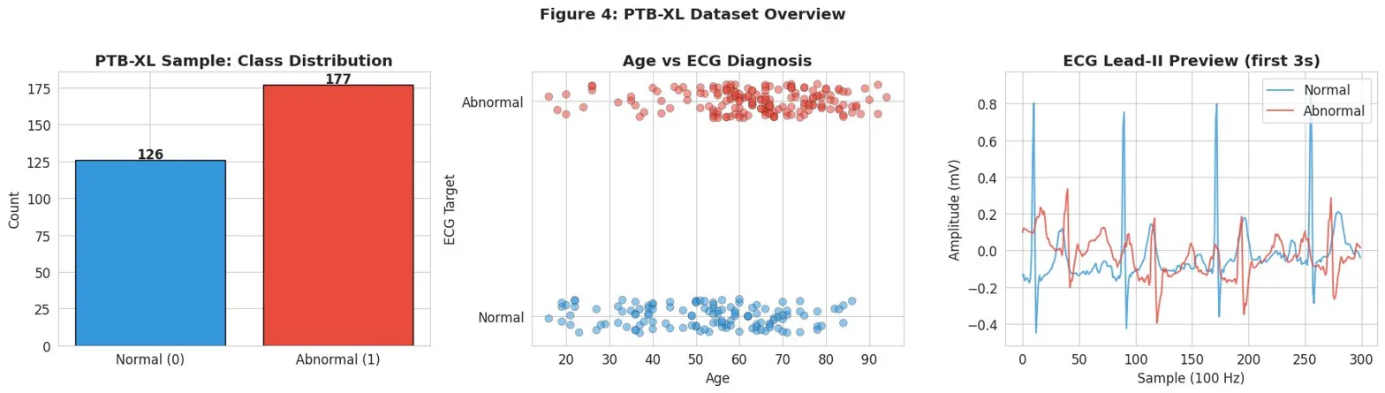
\includegraphics[width=\linewidth]{fig1_ptbxl_overview.png}
\caption{PTB-XL sample: class distribution, age versus diagnosis, and Lead-II traces (first 3~s).}
\label{fig:ptbxl}
\end{figure}

\subsection{ECG Feature Extraction}
Each Lead-II signal (1{,}000 samples at 100~Hz) is converted to the long format expected by tsfresh~\cite{christ2018} and processed with \texttt{EfficientFCParameters}, which yields 777 descriptors: time-domain statistics, autocorrelation, trend, entropy, spectral (FFT, Welch) and non-linear measures (c3, CID-CE, time-reversal asymmetry). tsfresh is suitable for fixed-length 10-s segments because its features are computed over the whole window and do not require beat segmentation~\cite{christ2018}. A VarianceThreshold filter ($\tau=0.01$) leaves 568 descriptors (in v4 this filter was fitted on all records; in this revision it is fitted inside each training fold).

\subsection{Datasets Used in This Study}
Table~\ref{tab:mapping} maps each dataset to its rows, features, label and the models trained on it (reviewer request).

\begin{table}[!t]
\centering\scriptsize
\caption{Dataset-to-model mapping.}
\label{tab:mapping}
\setlength{\tabcolsep}{2pt}
\begin{adjustbox}{max width=\linewidth}
\begin{tabular}{>{\raggedright\arraybackslash}p{1.15cm}>{\raggedright\arraybackslash}p{1.0cm}>{\raggedright\arraybackslash}p{1.35cm}>{\raggedright\arraybackslash}p{1.2cm}>{\raggedright\arraybackslash}p{2.55cm}}
\toprule
Dataset & Rows & Features & Label & Used for / models\\
\midrule
D1 Cleveland & 303 & 13 clinical & CAD (num$>$0) & Clinical-only baseline; LR, SVM, RF, XGB, GBM, voting, MLP\\
D3 Cleveland & 303 & 13 clinical + 23 ECG-proxy & CAD & Proposed system; all ablations (Sec.~VI-A--I)\\
D2 PTB-XL & 303 (1,212) & 568 tsfresh (Lead II) & ECG normal vs.\ abnormal & Parallel ECG benchmark (Sec.~VI-J); not fused with D1/D3\\
External & 294, 123, 200 & as D1/D3 & CAD & Test only (Sec.~VI-G)\\
\bottomrule
\end{tabular}
\end{adjustbox}
\end{table}

\section{Proposed Methodology}
\subsection{Pipeline Overview}
Fig.~\ref{fig:pipeline} shows the MultiCardioFusion pipeline. The clinical table (D1) is enriched with ECG-proxy features derived from the same patients' resting-ECG and exercise-test measurements (D3, Section~IV-D). Feature fusion with tree ensembles, a soft-voting ensemble and dual-branch neural networks are then trained and compared, and TreeSHAP explains the XGBoost member \emph{post hoc}. The PTB-XL branch (D2) is trained and evaluated separately with its own labels (Table~\ref{tab:mapping}).

\begin{figure}[!t]
\centering
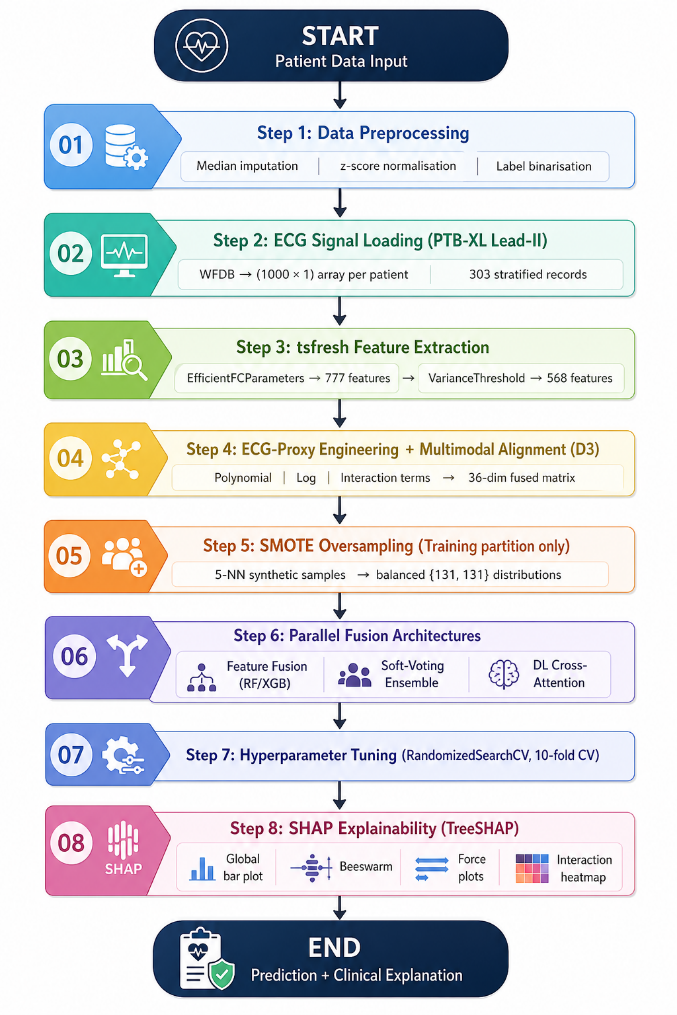
\includegraphics[width=0.78\linewidth]{fig2_pipeline.png}
\caption{MultiCardioFusion pipeline (as in v4). In this revision steps 1, 3, 4 and 5 are fitted inside each training fold (Algorithm~\ref{alg:train}).}
\label{fig:pipeline}
\end{figure}

\subsection{Algorithms}
The single MCF-BiModNet algorithm of v4 mixed a network forward pass with resampling, ensembling and explanation, which happen at different stages. It is split here into three algorithms: feature construction (Alg.~\ref{alg:proxy}), training and evaluation (Alg.~\ref{alg:train}) and post-hoc explanation (Alg.~\ref{alg:shap}). SHAP is \emph{not} part of prediction.

\begin{algorithm}[!t]
\caption{ECG-proxy feature construction (row-wise, no fitted parameters)}
\label{alg:proxy}
\begin{algorithmic}[1]
\Require imputed clinical vector $x\in\mathbb{R}^{13}$
\State $e \gets (\text{restecg}, \text{oldpeak}, \text{slope}, \text{thalach}, \text{exang})$ \Comment{5 raw ECG-linked}
\State append polynomial, interaction, log, ratio, threshold, HR-reserve and ischaemia terms (Section~IV-D) \Comment{18 derived}
\State \Return $[x;\, e] \in \mathbb{R}^{36}$
\end{algorithmic}
\end{algorithm}

\begin{algorithm}[!t]
\caption{Training and evaluation (repeated stratified CV)}
\label{alg:train}
\begin{algorithmic}[1]
\Require raw data $(X, y)$ with missing values; $R$ repeats, $K$ folds; fixed hyper-parameters $\theta$
\For{$r = 1..R$, $k = 1..K$}
  \State split into training $\mathcal{T}$ and test $\mathcal{V}$ (stratified)
  \State fit median imputer on $\mathcal{T}$; apply to $\mathcal{T}, \mathcal{V}$
  \State build features with Alg.~\ref{alg:proxy}; fit StandardScaler on $\mathcal{T}$
  \State resample $\mathcal{T}$ only (e.g.\ SMOTE, $k=5$)
  \State fit XGB, SVM, GBM, RF with $\theta$; $\bar P(x)=\frac14\sum_m P_m(x)$
  \State record AUC, accuracy, sensitivity, specificity, F1, Brier on $\mathcal{V}$
\EndFor
\State \Return fold metrics and paired differences with corrected CIs (Section~IV-G)
\end{algorithmic}
\end{algorithm}

\begin{algorithm}[!t]
\caption{Post-hoc interpretation (not used for prediction)}
\label{alg:shap}
\begin{algorithmic}[1]
\Require fitted XGBoost member $f$, transformed test features $Z_{\mathcal{V}}$
\State $\phi \gets \text{TreeSHAP}(f, Z_{\mathcal{V}})$; global importance $\bar\phi_j=\text{mean}|\phi_{\cdot j}|$
\State repeat over folds and seeds; report rank stability and agreement with permutation importance
\end{algorithmic}
\end{algorithm}

\subsection{Mathematical Formulation}
\textbf{SMOTE.} For a minority sample $x_i$, SMOTE~\cite{chawla2002} creates $\tilde x = x_i + \lambda(\hat x - x_i)$ with $\hat x$ one of the $k=5$ nearest minority neighbours and $\lambda\sim U(0,1)$. Interpolation stays within the convex hull of observed patients, but on mixed data it produces non-integer categorical codes and, when applied after feature derivation, derived features that no longer match their inputs (Section~VI-C). We therefore also evaluate SMOTE-NC~\cite{chawla2002} and resampling of the raw rows before feature derivation.

\textbf{Cross-attention with sequence length 1.} MCF-BiModNet reshapes each 32-dimensional branch output to a sequence of length $L=1$ and applies $\mathrm{Attention}(Q,K,V)=\mathrm{softmax}(QK^\top/\sqrt{d_k})V$ with $Q=W_Q h_{\text{ecg}}$, $K=W_K h_{\text{clin}}$, $V=W_V h_{\text{clin}}$. With one key, the softmax is taken over a single score, so the attention weight is exactly 1 for every head and every input. The block therefore reduces to
\begin{equation}
\mathrm{MultiHead}(h_{\text{ecg}}, h_{\text{clin}}) = W_O\,(W_V h_{\text{clin}} + b_V) + b_O ,
\end{equation}
a linear map of the clinical branch that does not depend on the ECG ``query''. We verify this numerically and compare the architecture with an explicit linear layer and with a \emph{token-level} variant in which every feature is a token, so that ECG-proxy tokens attend over 13 clinical tokens and the softmax is non-trivial (Section~VI-I).

\textbf{Soft voting.} Each base classifier $c_m$ outputs $P_m(x)\in[0,1]$; the ensemble predicts $\bar P(x) = \frac1M\sum_m P_m(x)$ and $\hat y = \mathbb{1}[\bar P(x)\geq 0.5]$. We compare soft voting with hard voting and with stacking, whose logistic meta-learner learns the member weights.

\textbf{TreeSHAP.} $\phi_j = \sum_{S\subseteq F\setminus\{j\}} \frac{|S|!(|F|-|S|-1)!}{|F|!}\,[f(S\cup\{j\}) - f(S)]$, computed exactly for tree ensembles in $O(TLD^2)$~\cite{lundberg2018tree}.

\subsection{ECG-Proxy Feature Engineering}
From the five ECG-related Cleveland variables (restecg, oldpeak, slope, thalach, exang) we derive 18 additional terms:
\emph{polynomial} oldpeak$^2$, thalach$^2$;
\emph{interactions} oldpeak$\times$slope, thalach$\times$exang, oldpeak$\times$thalach, restecg$\times$oldpeak, slope$\times$thalach;
\emph{log} $\log(1+\text{oldpeak})$, $\log(\text{thalach})$;
\emph{ratios} oldpeak/thalach, thalach/slope;
\emph{threshold flags} oldpeak$>$1, thalach$<$140, restecg$>$0, ``downslope'';
\emph{heart-rate reserve} thalach$-(220-\text{age})$ and its ratio to $220-\text{age}$;
and an \emph{ischaemia score} oldpeak$\cdot$(slope$+$1)$+$2$\cdot$exang.
Together with the five raw variables this gives a 23-column ECG-proxy block and a 36-column matrix D3. Two properties matter for interpretation. First, the five raw columns are exact copies of clinical columns, so D3 contains duplicates. Second, the v4 code defines ``downslope'' as slope $=2$, which in UCI coding is a \emph{flat} slope (downsloping is 3). Both are tested in Section~VI-A.

\subsection{Classifiers and Hyper-Parameters}
All models were implemented with scikit-learn~\cite{pedregosa2011}, XGBoost and imbalanced-learn~\cite{lemaitre2017}. The four ensemble members were tuned once by RandomizedSearchCV (10-fold) on the v4 training split: XGBoost~\cite{chen2016} (200 trees, depth 3, learning rate 0.01, column subsample 0.7), RBF-SVM~\cite{cortes1995} ($C=100$, $\gamma=0.001$), gradient boosting (200 trees, depth 3, learning rate 0.01) and random forest~\cite{breiman2001} (500 trees, depth 20, $\log_2$ features). In every experiment of Section~VI these values are \emph{fixed}, so all variants share the same tuning budget. Because they were tuned on data that overlaps the CV test folds, we also report fully nested tuning (Section~VI-D).

\subsection{Dual-Branch Neural Networks}
Each branch is Dense(64, ReLU)$\rightarrow$BatchNorm$\rightarrow$Dropout(0.4)$\rightarrow$Dense(32, ReLU)~\cite{ioffe2015,srivastava2014}. The clinical branch receives the 13 clinical columns and the ECG branch the 23 proxy columns. The branches are combined by concatenation, by multi-head cross-attention with $L=1$ (4 heads, $d_k=8$, residual to the ECG branch; the v4 architecture), by a linear layer (its equivalent), or by token-level cross-attention, in which each feature is embedded as its own token as in the FT-Transformer~\cite{gorishniy2021}. A Dense(16, ReLU)$\rightarrow$sigmoid head follows. Training uses Adam~\cite{kingma2015} (learning rate $10^{-3}$, batch 16, at most 200 epochs) with early stopping (patience 15, best weights restored) and learning-rate halving (patience 7) on a 20\% validation split of the training fold. \revnote{Note: the v4 notebook trained only a clinical-only MLP, so the cross-attention results reported in v4 had no corresponding code; the networks evaluated here were implemented for this revision.}

\subsection{Evaluation Protocol}
\textbf{Primary protocol.} All results in Section~VI use repeated stratified 10-fold CV with $R=5$ repeats (50 folds; 30 folds for the costlier neural and robustness experiments), with identical splits for every variant (Algorithm~\ref{alg:train}). AUC is the primary metric; sensitivity matters most clinically because a missed CAD case costs more than a false alarm. We also report specificity, F1, the Brier score and the calibration slope (ideal 1)~\cite{vancalster2019}.

\textbf{Uncertainty and tests.} Fold scores from repeated CV are not independent because training sets overlap, and a naive $t$-interval is too narrow. For a metric or paired difference $d_1,\dots,d_n$ over $n$ folds we use the corrected resampled $t$-statistic of Nadeau and Bengio~\cite{nadeau2003,bouckaert2004}:
\begin{equation}
t=\frac{\bar d}{\sqrt{\left(\frac1n+\frac{n_{\text{test}}}{n_{\text{train}}}\right)\hat\sigma^2_d}},
\end{equation}
with $n-1$ degrees of freedom and $n_{\text{test}}/n_{\text{train}}=1/9$, and report the matching 95\% CI. P-values within a table are adjusted with the Holm procedure~\cite{holm1979}. For external sites and subgroups we use 2{,}000 bootstrap resamples of patients. A label-permutation test~\cite{ojala2010} checks performance against chance.

\textbf{Hold-out.} For comparability with v4 we also report the 80/20 stratified hold-out (242/61 patients, seed 42), and its sensitivity to the choice of split (Section~VI-D).

\section{Baseline and Fusion Results}
\subsection{Unimodal Baselines (v4 protocol)}
Table~\ref{tab:unimodal} reproduces the v4 unimodal baselines. \revnote{These were computed by 10-fold CV \emph{on the SMOTE-balanced training partition}, so synthetic patients appear in the test folds and the scores are optimistic (Section~VI-D quantifies this bias). Leak-free values under the controlled protocol are given in Table~\ref{tab:e1}: the clinical-only soft-voting system reaches AUC \clinAUC{} \clinAUCci{}, and clinical-only logistic regression without any resampling reaches \clinLRAUCval{}.} ECG-only scores use PTB-XL labels and are not comparable with Cleveland scores (Section~III-C).

\begin{table}[!t]
\centering\scriptsize
\caption{Unimodal baselines from v4 (10-fold CV on the SMOTE-balanced training partition; optimistic, see text).}
\label{tab:unimodal}
\setlength{\tabcolsep}{2.5pt}
\begin{tabular}{llccccc}
\toprule
Data & Model & Acc. & AUC & F1 & Prec. & Rec.\\
\midrule
Clinical & Logistic regression & 0.832 & 0.894 & 0.830 & 0.849 & 0.818\\
Clinical & SVM (RBF) & 0.817 & 0.889 & 0.808 & 0.857 & 0.771\\
Clinical & Random forest & 0.813 & 0.904 & 0.810 & 0.835 & 0.793\\
Clinical & XGBoost & 0.809 & 0.882 & 0.812 & 0.815 & 0.817\\
\midrule
ECG (PTB-XL) & Logistic regression & 0.797 & 0.871 & 0.781 & 0.845 & 0.730\\
ECG (PTB-XL) & SVM (RBF) & 0.824 & 0.910 & 0.820 & 0.823 & 0.826\\
ECG (PTB-XL) & Random forest & 0.831 & 0.912 & 0.823 & 0.849 & 0.807\\
ECG (PTB-XL) & XGBoost & 0.790 & 0.898 & 0.773 & 0.828 & 0.737\\
\bottomrule
\end{tabular}
\end{table}

\subsection{Fusion Results Reported in v4}
Table~\ref{tab:v4fusion} lists the v4 fusion results \emph{with their actual protocols}. The v4 table presented all rows as hold-out results. In fact the first four rows were CV means on the SMOTE-balanced training partition, and the ``MCF-BiModNet XGB'' and ``Soft-Voting'' rows were the same soft-voting model. On the seed-42 hold-out the soft-voting model correctly identified 26 of 28 CAD patients and 28 of 33 non-CAD patients (Fig.~\ref{fig:eval}).

\begin{table}[!t]
\centering\scriptsize
\caption{v4 fusion results with corrected protocol labels.}
\label{tab:v4fusion}
\setlength{\tabcolsep}{2.5pt}
\begin{tabular}{lcccc}
\toprule
Model & Protocol & Acc. & AUC & Rec.\\
\midrule
Feature fusion -- RF & CV, SMOTE train set & 0.794 & 0.869 & 0.756\\
Feature fusion -- XGB & CV, SMOTE train set & 0.809 & 0.877 & 0.824\\
Soft voting (untuned) & CV, SMOTE train set & 0.821 & 0.891 & 0.801\\
Stacking & CV, SMOTE train set & 0.829 & 0.894 & 0.817\\
Clinical MLP (labelled ``DL dual-branch'') & hold-out (61) & 0.803 & 0.882 & 0.786\\
Tuned soft voting (``MCF-BiModNet'') & hold-out (61) & 0.885 & 0.954 & 0.929\\
\midrule
Tuned soft voting, fused & 10-fold CV (303) & 0.815 & -- & --\\
Tuned XGB, clinical vs.\ fused & 10-fold CV (303) & 0.815 vs.\ 0.815 & -- & --\\
\bottomrule
\end{tabular}
\end{table}

\begin{figure}[!t]
\centering
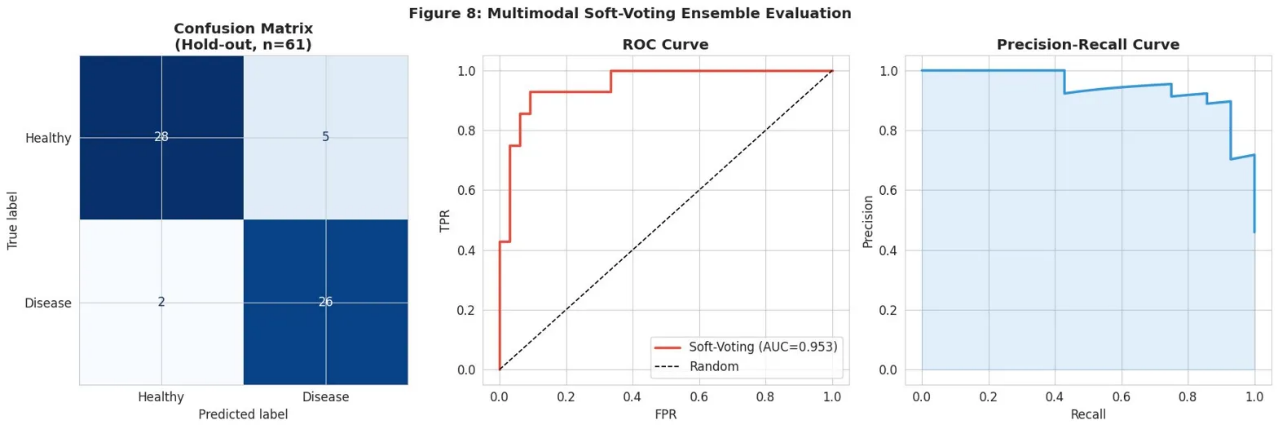
\includegraphics[width=\linewidth]{fig3_evaluation.png}
\caption{v4 soft-voting model on the seed-42 hold-out: confusion matrix, ROC and precision--recall curves. Section~VI-D shows that this split is unusually favourable.}
\label{fig:eval}
\end{figure}

\subsection{What the v4 Numbers Do and Do Not Show}
The v4 manuscript reported a ``+7.04 pp'' fusion gain. It was computed as the fused model's \emph{hold-out} accuracy (0.8852) minus the clinical XGBoost's \emph{10-fold CV} accuracy (0.8148), two numbers obtained under different protocols. Under the same protocol the v4 notebook itself found identical CV accuracy for clinical and fused XGBoost (0.8148 vs.\ 0.8148; paired $t=0$, $p=1.00$; McNemar $\chi^2=0.125$, $p=0.72$). Section~VI re-examines this and every other component claim under one controlled protocol.

\section{Extended Ablation Study}
This section is new in the revision. All experiments use the protocol of Section~IV-G: raw data, all preprocessing inside training folds, identical splits and fixed hyper-parameters for every variant, paired differences with corrected 95\% CIs, and Holm-adjusted p-values. In total \nVariants{} configurations were evaluated. Code and all result tables are in the accompanying notebook (Section~17B) and repository.

\begin{table*}[!t]
\centering
\scriptsize
\caption{Component ablation under the controlled protocol (5$\times$10-fold repeated CV, 50 paired folds, fixed hyper-parameters, all preprocessing inside folds). $\Delta$AUC is paired against the full system; CIs use the Nadeau--Bengio correction.}
\label{tab:e1}
\setlength{\tabcolsep}{3pt}
\begin{adjustbox}{max width=\linewidth}
\begin{tabular}{lcccccccc}
\toprule
Variant & AUC [95\% CI] & Acc. & Sens. & Spec. & F1 & Brier & $\Delta$AUC [95\% CI] & $p_{\mathrm{Holm}}$ \\
\midrule
Full system (clinical + ECG-proxy, SMOTE, soft voting) & 0.902 [0.858, 0.945] & 0.823 & 0.773 & 0.867 & 0.799 & 0.127 & -- & -- \\
\midrule
$-$ ECG-proxy block (clinical only) & 0.906 [0.864, 0.947] & 0.826 & 0.789 & 0.858 & 0.805 & 0.126 & +0.004 [-0.009, +0.017] & 1.000 \\
$-$ clinical block (ECG-proxy only) & 0.813 [0.758, 0.867] & 0.769 & 0.708 & 0.820 & 0.737 & 0.175 & -0.089 [-0.132, -0.046] & 0.003 \\
\midrule
$-$ duplicated raw proxy columns & 0.902 [0.858, 0.946] & 0.827 & 0.771 & 0.874 & 0.801 & 0.126 & +0.000 [-0.004, +0.005] & 1.000 \\
$-$ polynomial terms & 0.902 [0.858, 0.945] & 0.828 & 0.777 & 0.872 & 0.804 & 0.127 & +0.000 [-0.004, +0.004] & 1.000 \\
$-$ interaction terms & 0.902 [0.858, 0.946] & 0.822 & 0.773 & 0.864 & 0.798 & 0.126 & +0.001 [-0.004, +0.005] & 1.000 \\
$-$ log transforms & 0.902 [0.858, 0.945] & 0.827 & 0.774 & 0.873 & 0.803 & 0.127 & -0.000 [-0.004, +0.004] & 1.000 \\
$-$ ratio features & 0.901 [0.857, 0.945] & 0.825 & 0.781 & 0.863 & 0.803 & 0.127 & -0.001 [-0.006, +0.005] & 1.000 \\
$-$ threshold flags & 0.900 [0.858, 0.943] & 0.823 & 0.768 & 0.869 & 0.797 & 0.127 & -0.001 [-0.009, +0.006] & 1.000 \\
$-$ HR-reserve features & 0.901 [0.857, 0.944] & 0.826 & 0.780 & 0.866 & 0.803 & 0.127 & -0.001 [-0.006, +0.004] & 1.000 \\
$-$ ischaemia composite & 0.902 [0.858, 0.945] & 0.826 & 0.774 & 0.869 & 0.801 & 0.127 & +0.000 [-0.005, +0.006] & 1.000 \\
downslope coding fixed (slope==3) & 0.902 [0.858, 0.946] & 0.823 & 0.776 & 0.864 & 0.800 & 0.127 & +0.000 [-0.003, +0.004] & 1.000 \\
\midrule
$-$ SMOTE (no resampling) & 0.900 [0.855, 0.945] & 0.834 & 0.763 & 0.895 & 0.806 & 0.128 & -0.002 [-0.009, +0.006] & 1.000 \\
\midrule
$-$ soft voting $\rightarrow$ XGBoost only & 0.895 [0.850, 0.939] & 0.821 & 0.771 & 0.863 & 0.796 & 0.132 & -0.007 [-0.020, +0.006] & 1.000 \\
$-$ soft voting $\rightarrow$ SVM only & 0.905 [0.862, 0.949] & 0.840 & 0.815 & 0.861 & 0.823 & 0.121 & +0.004 [-0.015, +0.023] & 1.000 \\
$-$ soft voting $\rightarrow$ GBM only & 0.884 [0.840, 0.927] & 0.801 & 0.757 & 0.839 & 0.775 & 0.139 & -0.018 [-0.034, -0.002] & 0.558 \\
$-$ soft voting $\rightarrow$ RF only & 0.880 [0.831, 0.929] & 0.817 & 0.771 & 0.856 & 0.793 & 0.139 & -0.022 [-0.041, -0.002] & 0.510 \\
$-$ soft voting $\rightarrow$ logistic regression & 0.898 [0.853, 0.942] & 0.838 & 0.823 & 0.851 & 0.824 & 0.125 & -0.004 [-0.025, +0.017] & 1.000 \\
soft $\rightarrow$ hard (majority) voting & 0.869 [0.818, 0.920] & 0.812 & 0.796 & 0.825 & 0.793 & 0.147 & -0.032 [-0.053, -0.011] & 0.067 \\
soft voting $\rightarrow$ stacking (LR meta-learner) & 0.902 [0.857, 0.946] & 0.824 & 0.783 & 0.859 & 0.802 & 0.124 & -0.000 [-0.005, +0.005] & 1.000 \\
\midrule
Clinical only, no SMOTE, logistic regression & 0.904 [0.862, 0.946] & 0.835 & 0.794 & 0.871 & 0.814 & 0.123 & +0.003 [-0.017, +0.022] & 1.000 \\
\bottomrule
\end{tabular}
\end{adjustbox}
\end{table*}


\subsection{Component Ablation (RQ1, RQ2)}
Table~\ref{tab:e1} and Fig.~\ref{fig:a1} remove one component at a time. Under leak-free repeated CV the full system reaches AUC \fullAUC{} \fullAUCci{}, accuracy \fullAcc{}, sensitivity \fullSens{} and specificity \fullSpec{}. These figures are clearly lower than the v4 hold-out values (0.9535, 0.8852, 0.9286).

\textbf{ECG-proxy block.} Removing the entire proxy block (clinical only) changes AUC by \dClinAUC{} and accuracy by \dClinAcc{}~pp; the clinical-only system is numerically \emph{slightly better}. No individual feature group (polynomial, interaction, log, ratio, threshold, HR-reserve, ischaemia composite or the duplicated raw columns) changes AUC by more than \engMaxAbs{}. Correcting the ``downslope'' coding has no measurable effect. On its own, the proxy block is informative but clearly weaker than the clinical variables (proxy-only $\Delta$AUC \dProxyOnlyAUC{}, $p_{\text{Holm}}=\pProxyOnly{}$).

\textbf{SMOTE.} Removing SMOTE changes AUC by \dNoSmoteAUC{} and accuracy by \dNoSmoteAcc{}~pp. The v4 claim that SMOTE removal causes the largest drop (``$\approx$3.3\%'') is not reproduced. Without resampling, specificity rises (\noSmoteSpec{}) and sensitivity falls slightly (\noSmoteSens{}), as expected when the training prior is no longer artificially balanced.

\textbf{Ensemble.} Random forest alone ($\Delta$AUC \dRfOnlyAUC{}) and GBM alone (\dGbmOnlyAUC{}) have lower AUC than soft voting. Their uncorrected CIs exclude zero, but neither difference is significant after Holm correction ($p_{\text{Holm}}=\pRfOnly{}$ and \pGbmOnly{}). Soft voting does not outperform an RBF-SVM alone (\dSvmOnlyAUC{}) or plain logistic regression (\dLRAUC{}). Hard voting has the lowest AUC (\dHardAUC{}, $p_{\text{Holm}}=\pHard{}$), partly by construction: a four-member vote yields only five distinct scores, which limits ranking-based metrics. Stacking matches soft voting (\dStackAUC{}). A clinical-only logistic regression without any resampling reaches AUC \clinLRAUCval{} ($\Delta$ \dClinLRAUC{}), statistically indistinguishable from the full system.

\begin{figure}[!t]
\centering
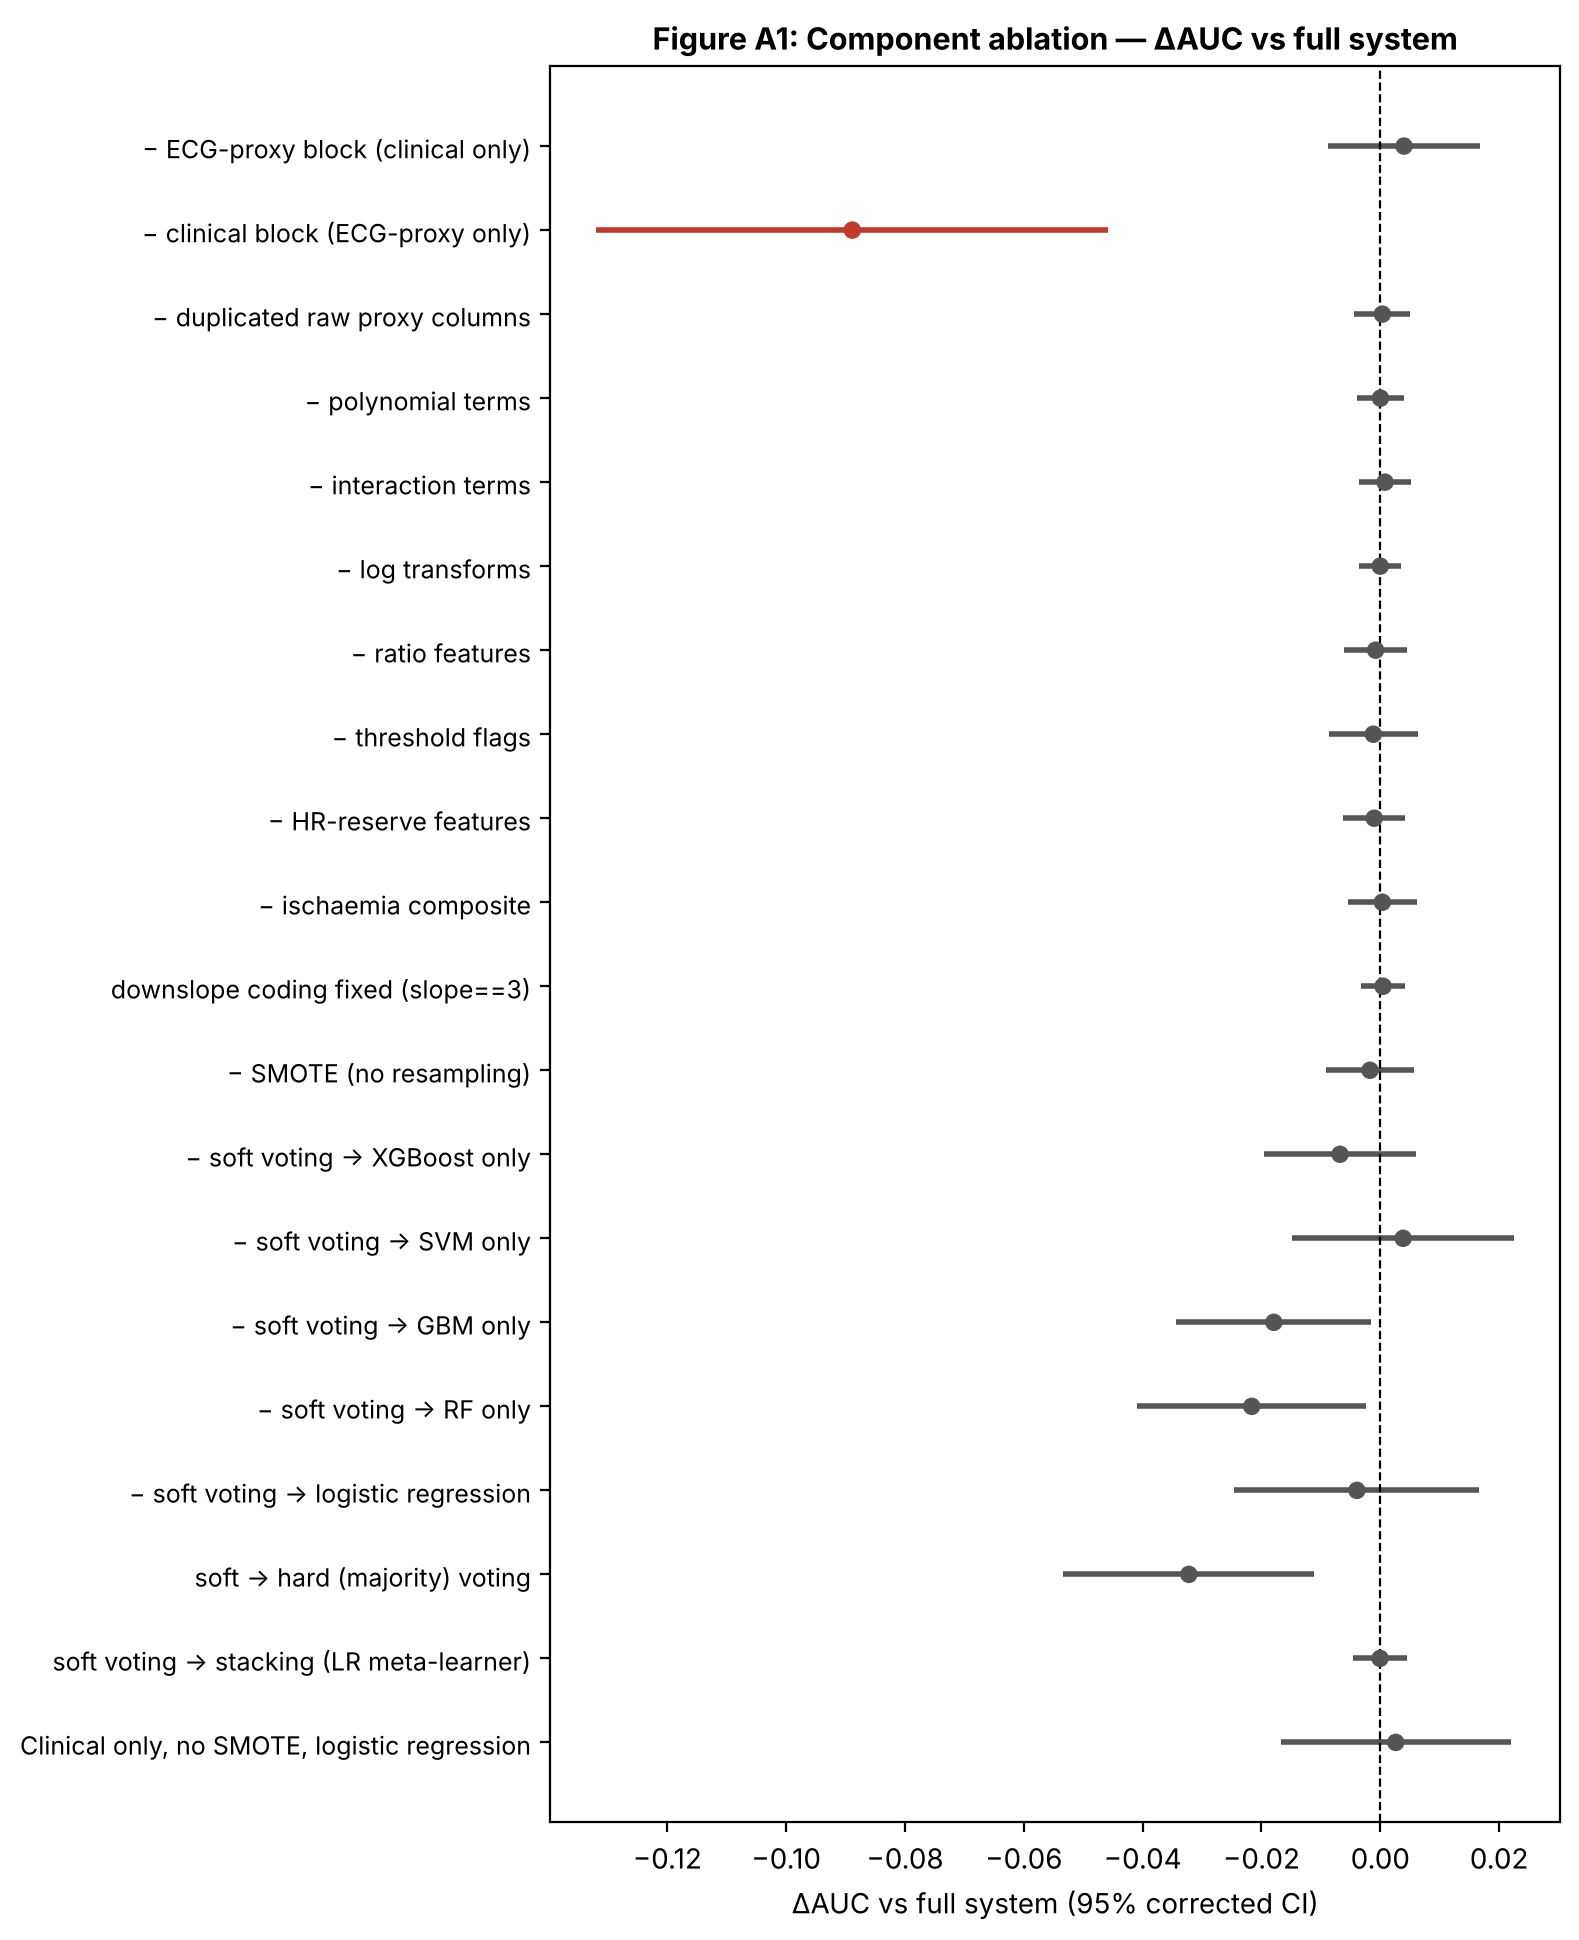
\includegraphics[width=\linewidth]{figA1_component_ablation.png}
\caption{Component ablation: paired $\Delta$AUC versus the full system with 95\% corrected CIs (grey = not significant after Holm correction).}
\label{fig:a1}
\end{figure}

\subsection{Control Experiments}
If the proxy block carried information beyond the clinical variables, it should outperform equally sized blocks of irrelevant features. Table~\ref{tab:e2} shows that it does not. Clinical + 18 engineered \emph{non-ECG} features (cholesterol, blood pressure and age transforms) reach AUC \nonecgAUC{}, clinical + 18 pure \emph{Gaussian-noise} columns \noiseAUC{}, and clinical + a \emph{row-shuffled} proxy block \shuffledAUC{}, all within the CI of the full system. This is expected: the proxy features are deterministic functions of variables the classifiers already see, and tree ensembles and RBF-SVMs can represent such products and ratios themselves. A label-permutation test confirms that the full system learns real signal (observed AUC \permObs{} versus \permNull{}$\pm$\permNullSd{} under \permN{} permutations, $p=\permP{}$, the smallest value attainable with \permN{} permutations).

\begin{table*}[!t]
\centering
\scriptsize
\caption{Control experiments: is the ECG-proxy block better than other added features?}
\label{tab:e2}
\setlength{\tabcolsep}{3pt}
\begin{adjustbox}{max width=\linewidth}
\begin{tabular}{lcccc}
\toprule
Feature set (soft voting, SMOTE) & AUC [95\% CI] & Acc. & $\Delta$AUC vs full & $p_{\mathrm{Holm}}$ \\
\midrule
Full system (clinical + ECG-proxy, SMOTE, soft voting) & 0.902 [0.858, 0.945] & 0.823 & -- & -- \\
Clinical only & 0.906 [0.864, 0.947] & 0.826 & +0.004 [-0.009, +0.017] & 1.000 \\
Clinical + 18 engineered non-ECG features & 0.903 [0.861, 0.946] & 0.822 & +0.002 [-0.016, +0.020] & 1.000 \\
Clinical + 18 Gaussian-noise features & 0.899 [0.855, 0.943] & 0.824 & -0.003 [-0.023, +0.018] & 1.000 \\
Clinical + row-shuffled ECG-proxy block & 0.897 [0.850, 0.944] & 0.826 & -0.004 [-0.020, +0.011] & 1.000 \\
Clinical + ECG-proxy + non-ECG features & 0.902 [0.859, 0.944] & 0.822 & +0.000 [-0.011, +0.012] & 1.000 \\
\bottomrule
\end{tabular}
\end{adjustbox}
\end{table*}


\subsection{Class-Imbalance Strategies}
Cleveland is only mildly imbalanced (54.1\%/45.9\%), and Table~\ref{tab:e3} shows that the choice of strategy hardly matters: no correction, class weighting, random oversampling, SMOTE after or before feature derivation, SMOTE-NC~\cite{chawla2002}, Borderline-SMOTE~\cite{han2005borderline} and ADASYN~\cite{he2008adasyn} all lie within $\pm$0.005 AUC of each other, with no significant differences. SMOTE does, however, create implausible patients: in the first training fold \smoteNonInt{} of the synthetic rows carry non-integer categorical codes (e.g.\ chest-pain type 2.6), and when SMOTE is applied after feature derivation \smoteInconsistent{} of synthetic rows have oldpeak$^2$ differing from the square of their oldpeak by more than 5\%. Because it brings no measurable benefit here, we recommend class weighting or no correction for this dataset, and SMOTE-NC on raw rows where oversampling is required. Table~\ref{tab:counts} gives the class counts per partition.

\begin{table*}[!t]
\centering
\scriptsize
\caption{Class-imbalance strategies (full feature set, soft voting; resampling inside training folds only). Calibration slope: ideal 1; $>$1 means under-confident probabilities.}
\label{tab:e3}
\setlength{\tabcolsep}{3pt}
\begin{adjustbox}{max width=\linewidth}
\begin{tabular}{lcccccc}
\toprule
Imbalance strategy & AUC & Sens. & Spec. & Brier & Cal.\ slope & $\Delta$AUC [95\% CI] \\
\midrule
SMOTE after features (paper) & 0.902 & 0.773 & 0.867 & 0.127 & 1.37 & -- \\
No correction & 0.900 & 0.763 & 0.895 & 0.128 & 1.41 & -0.002 [-0.009, +0.006] \\
Class weighting (no resampling) & 0.901 & 0.768 & 0.882 & 0.127 & 1.42 & -0.001 [-0.007, +0.005] \\
Random oversampling & 0.897 & 0.771 & 0.867 & 0.129 & 1.40 & -0.005 [-0.013, +0.003] \\
SMOTE on raw rows $\rightarrow$ derive proxy & 0.899 & 0.774 & 0.867 & 0.128 & 1.36 & -0.003 [-0.010, +0.005] \\
SMOTE-NC on raw rows $\rightarrow$ derive proxy & 0.900 & 0.771 & 0.872 & 0.128 & 1.37 & -0.002 [-0.009, +0.005] \\
Borderline-SMOTE & 0.900 & 0.789 & 0.851 & 0.129 & 1.39 & -0.001 [-0.010, +0.008] \\
ADASYN & 0.903 & 0.779 & 0.868 & 0.126 & 1.45 & +0.001 [-0.006, +0.008] \\
\bottomrule
\end{tabular}
\end{adjustbox}
\end{table*}

\begin{table}[!t]
\centering
\scriptsize
\caption{Class counts per partition (H = healthy, D = disease). SMOTE is fitted on training rows only.}
\label{tab:counts}
\setlength{\tabcolsep}{3pt}
\begin{adjustbox}{max width=\linewidth}
\begin{tabular}{lccc}
\toprule
Partition & Train (H/D) & After SMOTE & Test (H/D) \\
\midrule
D1/D3 Cleveland (80/20 hold-out) & 131/111 & 131/131 & 33/28 \\
D1/D3 Cleveland (one 10-fold CV fold) & 147/125 & 147/147 & 17/14 \\
\bottomrule
\end{tabular}
\end{adjustbox}
\end{table}


\subsection{Evaluation Protocol and Leakage}
Table~\ref{tab:e4} quantifies protocol choices. Fitting imputation and scaling on all 303 patients (as in v4) has negligible effect here (AUC \leakPreAUC{}), because only six values are missing and the scaler's statistics hardly change. Applying SMOTE \emph{before} cross-validation, however, inflates AUC to \leakSmoteAUC{}, because synthetic neighbours of test patients enter the training folds. Errors of this kind could contribute to some very high accuracies reported in the literature, although we cannot tell which published studies, if any, are affected. Fully nested tuning of XGBoost (AUC \nestedAUC{}) performs similarly to the fixed Section-15 parameters (\fixedXgbAUC{}) and better than library defaults (\defaultXgbAUC{}), so the fixed parameters introduce no detectable optimism.

\begin{table*}[!t]
\centering
\scriptsize
\caption{Leakage and tuning protocol (5$\times$10-fold CV). Leaky rows are shown only to quantify the bias.}
\label{tab:e4}
\setlength{\tabcolsep}{3pt}
\begin{adjustbox}{max width=\linewidth}
\begin{tabular}{lccc}
\toprule
Protocol & AUC [95\% CI] & Accuracy [95\% CI] & Sensitivity [95\% CI] \\
\midrule
Leak-free CV (reference) & 0.902 [0.858, 0.945] & 0.823 [0.766, 0.881] & 0.773 [0.686, 0.860] \\
Leaky (a): preprocessing fitted on all rows & 0.902 [0.859, 0.945] & 0.823 [0.765, 0.881] & 0.773 [0.685, 0.861] \\
Leaky (b): SMOTE before CV & 0.916 [0.877, 0.955] & 0.838 [0.793, 0.884] & 0.794 [0.718, 0.870] \\
XGBoost, fixed Section-15 params & 0.895 [0.850, 0.939] & 0.821 [0.764, 0.877] & 0.771 [0.684, 0.859] \\
XGBoost, nested tuning (inner 3-fold) & 0.900 [0.859, 0.942] & 0.822 [0.767, 0.877] & 0.780 [0.695, 0.865] \\
XGBoost, library defaults & 0.875 [0.831, 0.919] & 0.789 [0.732, 0.847] & 0.749 [0.664, 0.834] \\
\bottomrule
\end{tabular}
\end{adjustbox}
\end{table*}


\textbf{Hold-out sensitivity.} The v4 headline numbers come from one 80/20 split (seed 42). Repeating the identical leak-free pipeline on \hoN{} random 80/20 splits (Table~\ref{tab:holdout}, Fig.~\ref{fig:a3}) gives a mean fused accuracy of \hoFuAcc{}, while seed 42 gives \hoFuAccSeed{}, the \hoFuAccPct{}th percentile. For fused AUC, seed 42 lies at the \hoFuAUCPct{}th percentile. The fused$-$clinical accuracy difference averages \hoDAcc{} across splits, so a single favourable split can produce an apparent gain of several points by chance. Single 61-patient hold-out results on this dataset should therefore always be accompanied by repeated-split or repeated-CV estimates.

\begin{table*}[!t]
\centering
\scriptsize
\caption{Sensitivity of the 61-patient hold-out estimate to the random split (leak-free pipeline). ``Pct. is the percentile of the seed-42 split used in the v4 paper.}
\label{tab:holdout}
\setlength{\tabcolsep}{3pt}
\begin{adjustbox}{max width=\linewidth}
\begin{tabular}{lccc}
\toprule
Metric & Mean (2.5--97.5\%) over random 80/20 splits & Seed 42 & Pct. \\
\midrule
Fused accuracy & 0.833 (2.5--97.5\%: 0.754--0.918) & 0.902 & 95 \\
Clinical accuracy & 0.831 (2.5--97.5\%: 0.738--0.902) & 0.869 & 81 \\
Fused $-$ clinical accuracy & 0.002 (2.5--97.5\%: -0.049--0.049) & 0.033 & 90 \\
Fused AUC & 0.904 (2.5--97.5\%: 0.832--0.955) & 0.96 & 99 \\
Clinical AUC & 0.911 (2.5--97.5\%: 0.840--0.960) & 0.948 & 90 \\
Fused $-$ clinical AUC & -0.007 (2.5--97.5\%: -0.034--0.017) & 0.012 & 94 \\
\bottomrule
\end{tabular}
\end{adjustbox}
\end{table*}


\begin{figure}[!t]
\centering
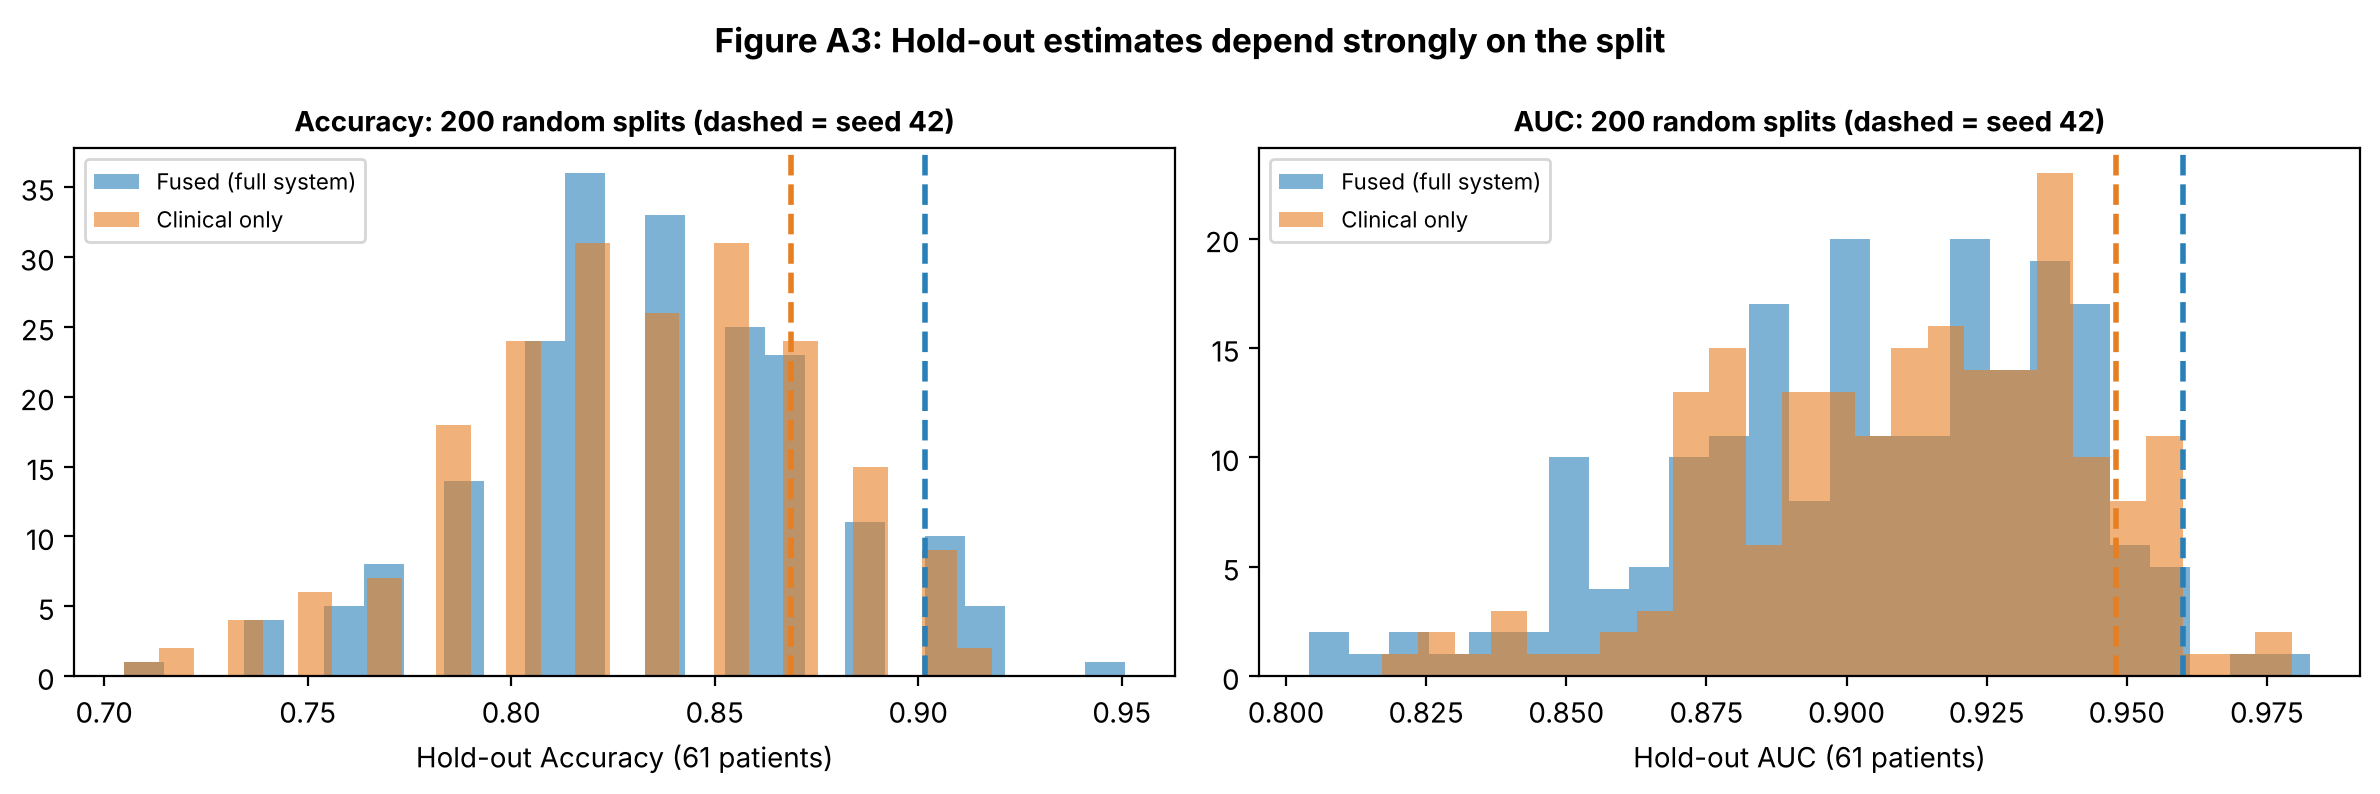
\includegraphics[width=\linewidth]{figA3_holdout_sensitivity.png}
\caption{Distribution of hold-out accuracy and AUC over \hoN{} random 80/20 splits; dashed lines mark the seed-42 split used in v4.}
\label{fig:a3}
\end{figure}

\subsection{Robustness and Edge Cases (RQ3)}
A proxy block could still be useful in harder conditions even if it adds nothing on clean data. Table~\ref{tab:e5} and Fig.~\ref{fig:a4} apply 16 perturbations identically to the fused and clinical-only systems: training label noise (5--20\%), missing values at test time or in both training and test data (10--30\%, MCAR), Gaussian measurement noise (0.25--1~SD), reduced training sets (25--75\%), and clinically motivated missing modalities. Across all scenarios $\Delta$AUC lies between \robMinD{} and \robMaxD{}, and \robNsig{} of \robN{} comparisons are significant after Holm correction. The proxy block does not make the model more robust to label noise (20\% noise: \robNoiseFu{} vs.\ \robNoiseCl{}) or to small training sets (25\%: \robSmallFu{} vs.\ \robSmallCl{}). The most clinically relevant edge case is a patient without angiography or a thallium scan (\texttt{ca}, \texttt{thal} unavailable), where ECG-derived information might be expected to matter most. Even there the fused and clinical systems perform equally (\robNoAngioFu{} vs.\ \robNoAngioCl{}; $\Delta$ \robNoAngioD{}). Removing the exercise test costs little (AUC \robNoExFu{}), whereas resting data alone (no exercise test, no angiography or thallium) drops AUC to \robRestFu{}. This identifies \texttt{ca}, \texttt{thal} and \texttt{cp} as the dominant information sources.

\begin{table*}[!t]
\centering
\scriptsize
\caption{Robustness and edge cases. Each perturbation is applied identically to the fused and the clinical-only system.}
\label{tab:e5}
\setlength{\tabcolsep}{3pt}
\begin{adjustbox}{max width=\linewidth}
\begin{tabular}{lccccc}
\toprule
Scenario (3$\times$10-fold CV) & AUC fused & AUC clin. & $\Delta$AUC [95\% CI] & $p_{\mathrm{Holm}}$ & Sens. fused / clin. \\
\midrule
Baseline (no perturbation) & 0.901 & 0.907 & -0.006 [-0.018, +0.006] & 1.000 & 0.780 / 0.787 \\
Training label noise 5\% & 0.894 & 0.906 & -0.011 [-0.025, +0.002] & 1.000 & 0.779 / 0.789 \\
Training label noise 10\% & 0.889 & 0.901 & -0.012 [-0.029, +0.005] & 1.000 & 0.791 / 0.787 \\
Training label noise 20\% & 0.863 & 0.877 & -0.014 [-0.033, +0.005] & 1.000 & 0.741 / 0.780 \\
Test-time missing values (MCAR) 10\% & 0.892 & 0.894 & -0.002 [-0.016, +0.012] & 1.000 & 0.753 / 0.741 \\
Test-time missing values (MCAR) 20\% & 0.876 & 0.880 & -0.004 [-0.017, +0.009] & 1.000 & 0.688 / 0.671 \\
Test-time missing values (MCAR) 30\% & 0.863 & 0.862 & +0.002 [-0.014, +0.017] & 1.000 & 0.633 / 0.616 \\
Missing values in train AND test 20\% & 0.878 & 0.880 & -0.002 [-0.016, +0.012] & 1.000 & 0.770 / 0.756 \\
Measurement noise $\sigma$=0.25$\times$SD (test) & 0.899 & 0.906 & -0.007 [-0.019, +0.005] & 1.000 & 0.782 / 0.789 \\
Measurement noise $\sigma$=0.5$\times$SD (test) & 0.901 & 0.904 & -0.003 [-0.017, +0.012] & 1.000 & 0.794 / 0.789 \\
Measurement noise $\sigma$=1.0$\times$SD (test) & 0.898 & 0.900 & -0.003 [-0.022, +0.017] & 1.000 & 0.789 / 0.785 \\
Training set reduced to 25\% & 0.872 & 0.882 & -0.010 [-0.029, +0.008] & 1.000 & 0.763 / 0.762 \\
Training set reduced to 50\% & 0.886 & 0.900 & -0.014 [-0.036, +0.008] & 1.000 & 0.777 / 0.794 \\
Training set reduced to 75\% & 0.896 & 0.909 & -0.013 [-0.028, +0.002] & 1.000 & 0.794 / 0.794 \\
No angiography/thallium (ca, thal unavailable) & 0.864 & 0.866 & -0.002 [-0.015, +0.012] & 1.000 & 0.767 / 0.760 \\
No exercise test (thalach, exang, oldpeak, slope) & 0.905 & 0.901 & +0.004 [-0.003, +0.012] & 1.000 & 0.782 / 0.775 \\
Resting data only (both unavailable) & 0.837 & 0.834 & +0.003 [-0.009, +0.015] & 1.000 & 0.784 / 0.770 \\
\bottomrule
\end{tabular}
\end{adjustbox}
\end{table*}


\begin{figure}[!t]
\centering
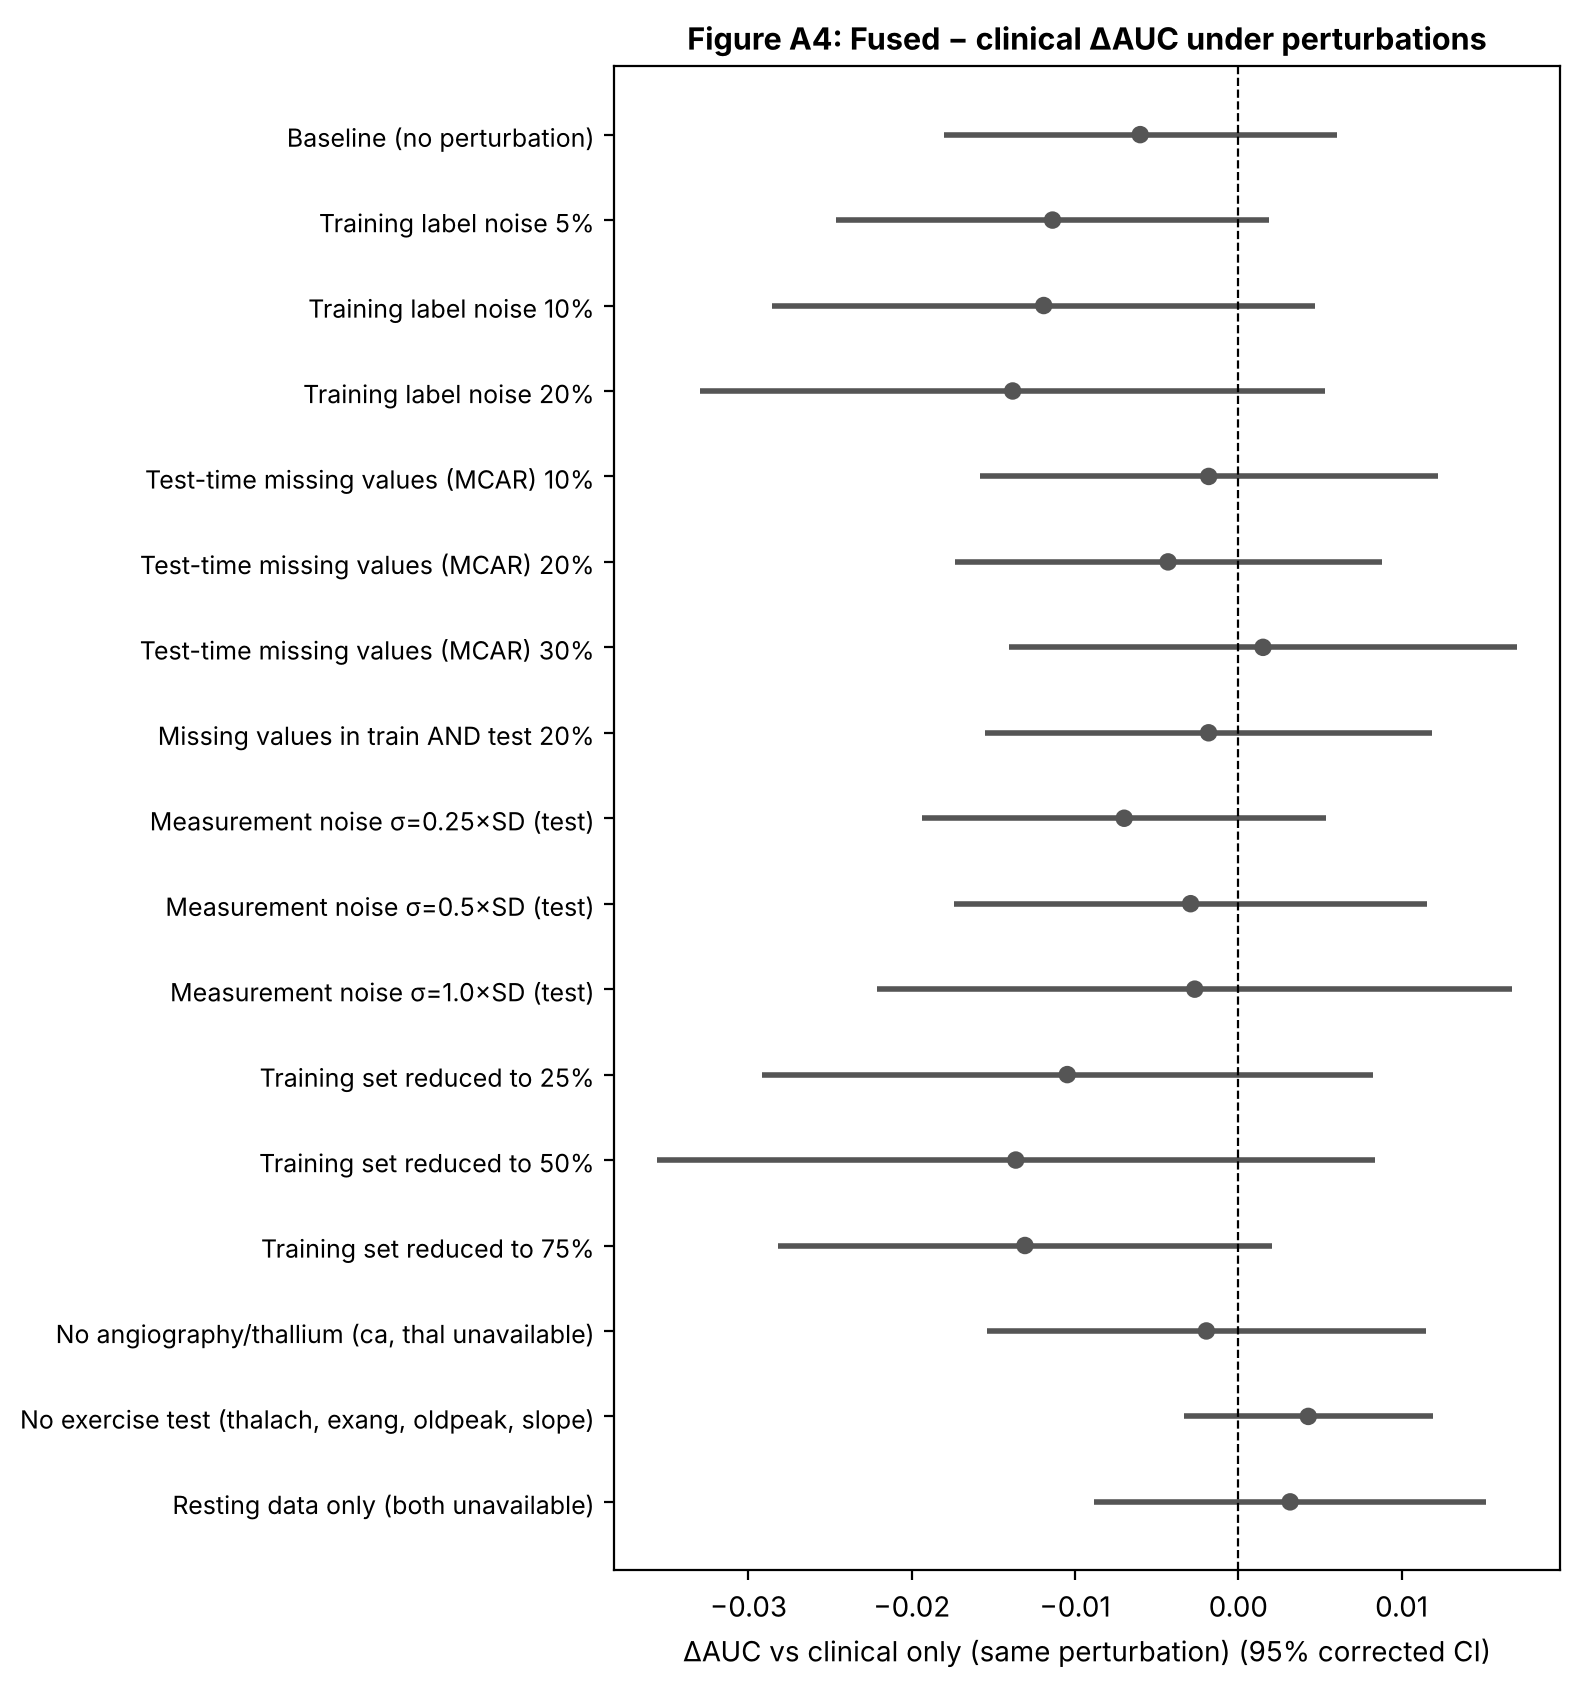
\includegraphics[width=\linewidth]{figA4_robustness.png}
\caption{Fused minus clinical-only $\Delta$AUC under each perturbation (3$\times$10-fold CV, paired).}
\label{fig:a4}
\end{figure}

\textbf{Subgroups.} Table~\ref{tab:subgroups} reports out-of-fold performance by sex, age, chest-pain type and resting ECG. The proxy block does not significantly help any subgroup; every subgroup $\Delta$AUC CI includes zero. Discrimination is similar in women and men but lower in patients aged $\geq$55 years than in younger patients, and lowest in patients with symptomatic chest pain (cp~1--3), where CAD is less prevalent and the dominant predictor \texttt{cp} carries less information. These are the groups in which the model would most need improvement before clinical use.

\begin{table}[!t]
\centering
\scriptsize
\caption{Subgroup performance (out-of-fold predictions averaged over 5 repeats; bootstrap CIs).}
\label{tab:subgroups}
\setlength{\tabcolsep}{3pt}
\begin{adjustbox}{max width=\linewidth}
\begin{tabular}{lccccc}
\toprule
Subgroup & n & Dis. & AUC fused & AUC clin. & $\Delta$AUC [95\% CI] \\
\midrule
All patients & 303 & 139 & 0.900 & 0.905 & -0.005 [-0.014, +0.003] \\
Female & 97 & 25 & 0.899 & 0.908 & -0.008 [-0.026, +0.007] \\
Male & 206 & 114 & 0.883 & 0.884 & -0.002 [-0.013, +0.009] \\
Age < 55 & 143 & 44 & 0.933 & 0.935 & -0.003 [-0.016, +0.013] \\
Age $\geq$ 55 & 160 & 95 & 0.853 & 0.858 & -0.005 [-0.018, +0.010] \\
Asymptomatic chest pain (cp=4) & 144 & 105 & 0.882 & 0.890 & -0.008 [-0.028, +0.008] \\
Symptomatic chest pain (cp=1--3) & 159 & 34 & 0.802 & 0.815 & -0.012 [-0.041, +0.014] \\
Normal resting ECG & 151 & 56 & 0.885 & 0.884 & +0.000 [-0.013, +0.014] \\
Abnormal resting ECG & 152 & 83 & 0.912 & 0.920 & -0.008 [-0.018, +0.001] \\
\bottomrule
\end{tabular}
\end{adjustbox}
\end{table}


\subsection{Ordinal Encoding and Calibration}
One-hot coding of \texttt{cp}, \texttt{restecg}, \texttt{slope} and \texttt{thal} gives AUC \calOnehotAUC{} for the full system (Table~\ref{tab:e6}), no different from ordinal coding, because the dominant tree and RBF members are insensitive to the coding. Calibration matters more for clinical use than a third decimal of AUC~\cite{vancalster2019}. The soft-voting ensemble has a calibration slope of \calFull{}: its probabilities are \emph{under-confident}, compressed towards 0.5 by averaging. The Brier score is \brierFull{}. Platt scaling moves the slope towards 1 (\calPlattSlope{}; Brier \calPlattBrier{}) without changing discrimination. Isotonic regression over-corrects (slope \calIsoSlope{}, i.e.\ over-confident; Brier \calIsoBrier{}), as is typical when a non-parametric calibrator is fitted on about 240 patients (Fig.~\ref{fig:a5}). In this cohort Platt scaling therefore performed better than isotonic regression. Any calibration should be re-estimated in the target population before clinical use. Equal voting weights are adequate: learned weights (stacking) give the same AUC.

\begin{table*}[!t]
\centering
\scriptsize
\caption{Ordinal versus one-hot encoding and probability calibration.}
\label{tab:e6}
\setlength{\tabcolsep}{3pt}
\begin{adjustbox}{max width=\linewidth}
\begin{tabular}{lcccc}
\toprule
Variant & AUC & Brier & Cal.\ slope & $\Delta$AUC [95\% CI] \\
\midrule
Full system (clinical + ECG-proxy, SMOTE, soft voting) & 0.902 & 0.127 & 1.37 & -- \\
One-hot cp/restecg/slope/thal (full system) & 0.903 & 0.127 & 1.39 & +0.002 [-0.007, +0.011] \\
One-hot cp/restecg/slope/thal (clinical only) & 0.907 & 0.126 & 1.35 & +0.006 [-0.009, +0.020] \\
Clinical only & 0.906 & 0.126 & 1.37 & +0.004 [-0.009, +0.017] \\
Platt-calibrated soft voting & 0.900 & 0.125 & 1.13 & -0.001 [-0.006, +0.004] \\
Isotonic-calibrated soft voting & 0.900 & 0.127 & 0.56 & -0.001 [-0.010, +0.008] \\
$-$ SMOTE (no resampling) & 0.900 & 0.128 & 1.41 & -0.002 [-0.009, +0.006] \\
\bottomrule
\end{tabular}
\end{adjustbox}
\end{table*}


\begin{figure}[!t]
\centering
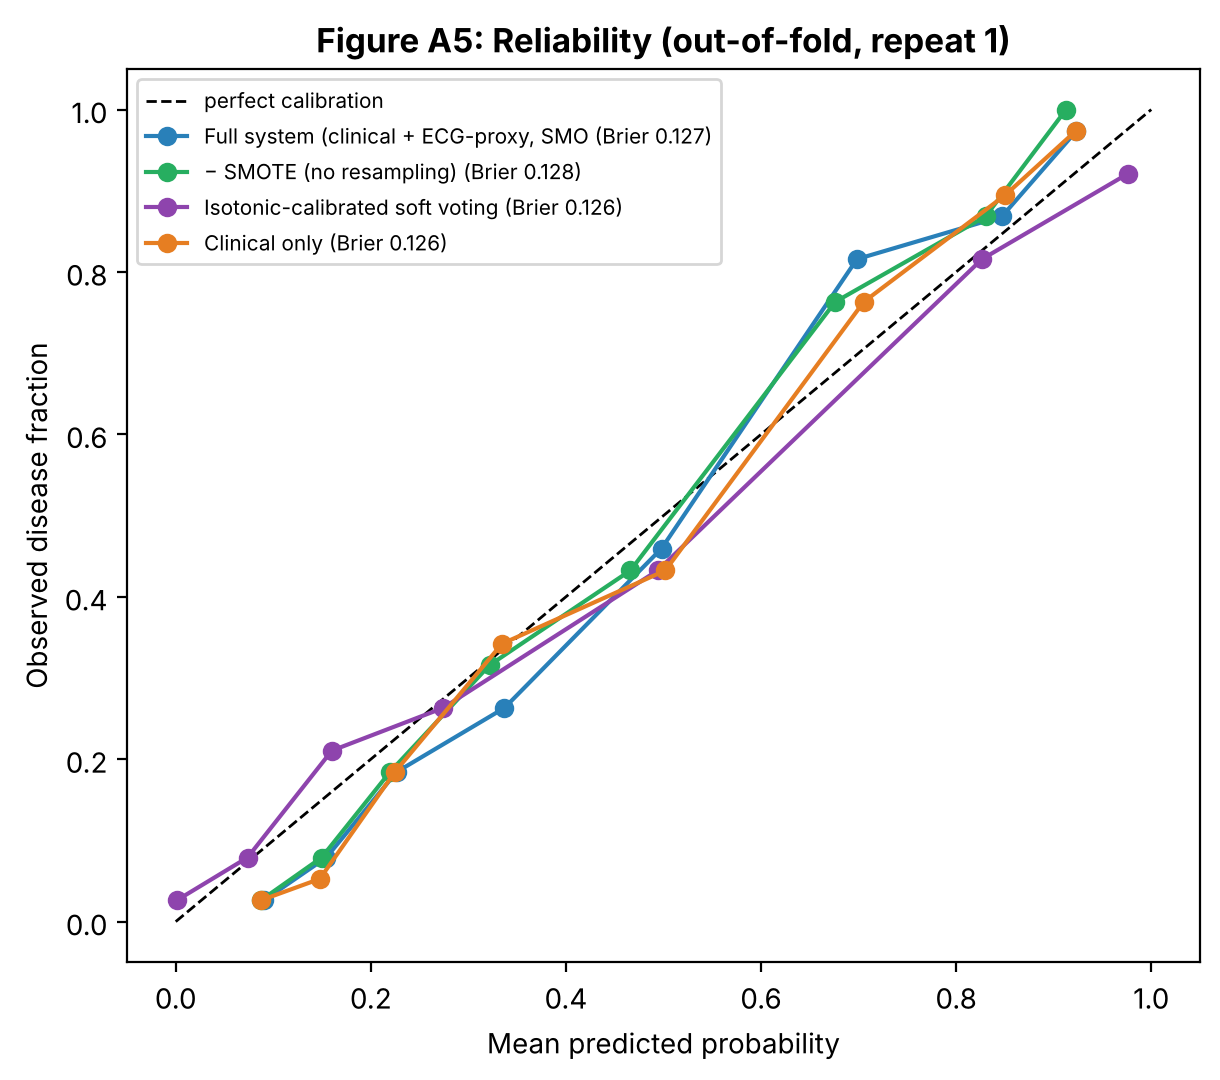
\includegraphics[width=0.85\linewidth]{figA5_calibration.png}
\caption{Reliability diagram of out-of-fold probabilities (repeat 1).}
\label{fig:a5}
\end{figure}

\subsection{External Validation on Three Further Hospitals (RQ3)}
All earlier results are internal to Cleveland. Table~\ref{tab:sites} shows that the three other UCI sites differ markedly from it. CAD prevalence ranges from 36\% (Hungary) to 94\% (Switzerland), and the two strongest Cleveland predictors are mostly unavailable: \texttt{ca} is missing for 96--99\% and \texttt{thal} for 42--90\% of patients. Models trained on all 303 Cleveland patients and applied unchanged (Table~\ref{tab:e7}, Fig.~\ref{fig:a6}) reach AUC \extHunFu{} in Hungary, \extSwiFu{} in Switzerland and \extVaFu{} at VA Long Beach (clinical-only: \extHunCl{}, \extSwiCl{}, \extVaCl{}). Fused and clinical-only models do not differ at any site (fused$-$clinical $\Delta$AUC with bootstrap CI: \extDeltaList{}).

A second edge case emerges here. When \texttt{ca} and \texttt{thal} are missing, median imputation fills them with Cleveland's medians (0 vessels, normal thallium), the values most typical of \emph{healthy} patients. Sensitivity therefore collapses at the external sites (Table~\ref{tab:e7}). Training without \texttt{ca}, \texttt{thal} and \texttt{slope} restores sensitivity to 0.77--0.85 and improves calibration (lower Brier) at the cost of specificity, and at VA it also improves AUC. A model should therefore be trained on the features that will actually be available at deployment rather than relying on imputation of its most important inputs. Cholesterol is recorded as 0~mg/dL for all 123 Swiss and 49 VA patients. Treating these values as missing rather than literally changes external AUC by at most 0.004, because cholesterol carries little weight in the model (\texttt{E7\_chol\_zero\_edge\_case.csv} in the repository).

\begin{table}[!t]
\centering
\scriptsize
\caption{Characteristics of the four UCI heart-disease sites (chol = 0 treated as missing).}
\label{tab:sites}
\setlength{\tabcolsep}{3pt}
\begin{adjustbox}{max width=\linewidth}
\begin{tabular}{lcccccc}
\toprule
Site & n & Prev. & ca miss. & thal miss. & slope miss. & chol miss. \\
\midrule
Cleveland & 303 & 45.9\% & 1\% & 1\% & 0\% & 0\% \\
Hungary & 294 & 36.1\% & 99\% & 90\% & 65\% & 8\% \\
Switzerland & 123 & 93.5\% & 96\% & 42\% & 14\% & 100\% \\
VA Long Beach & 200 & 74.5\% & 99\% & 83\% & 51\% & 28\% \\
\bottomrule
\end{tabular}
\end{adjustbox}
\end{table}

\begin{table*}[!t]
\centering
\scriptsize
\caption{External validation: trained on all 303 Cleveland patients, tested unchanged on three other hospitals.}
\label{tab:e7}
\setlength{\tabcolsep}{3pt}
\begin{adjustbox}{max width=\linewidth}
\begin{tabular}{llcccc}
\toprule
Site & Model (trained on Cleveland) & AUC [95\% CI] & Sens. & Spec. & Brier \\
\midrule
Hungary & Clinical only & 0.886 [0.844, 0.927] & 0.557 & 0.963 & 0.143 \\
Hungary & Clinical, without ca/thal/slope & 0.885 [0.844, 0.925] & 0.774 & 0.830 & 0.135 \\
Hungary & Fused (full system) & 0.889 [0.847, 0.931] & 0.670 & 0.931 & 0.133 \\
Hungary & Fused, without ca/thal/slope & 0.883 [0.841, 0.925] & 0.774 & 0.846 & 0.136 \\
Switzerland & Clinical only & 0.785 [0.596, 0.946] & 0.548 & 0.875 & 0.262 \\
Switzerland & Clinical, without ca/thal/slope & 0.792 [0.615, 0.951] & 0.817 & 0.625 & 0.150 \\
Switzerland & Fused (full system) & 0.772 [0.552, 0.959] & 0.574 & 0.750 & 0.250 \\
Switzerland & Fused, without ca/thal/slope & 0.771 [0.560, 0.941] & 0.800 & 0.625 & 0.154 \\
VA Long Beach & Clinical only & 0.721 [0.635, 0.803] & 0.463 & 0.784 & 0.261 \\
VA Long Beach & Clinical, without ca/thal/slope & 0.751 [0.672, 0.828] & 0.846 & 0.451 & 0.168 \\
VA Long Beach & Fused (full system) & 0.709 [0.622, 0.790] & 0.510 & 0.784 & 0.255 \\
VA Long Beach & Fused, without ca/thal/slope & 0.754 [0.674, 0.826] & 0.839 & 0.490 & 0.176 \\
\bottomrule
\end{tabular}
\end{adjustbox}
\end{table*}


\begin{figure}[!t]
\centering
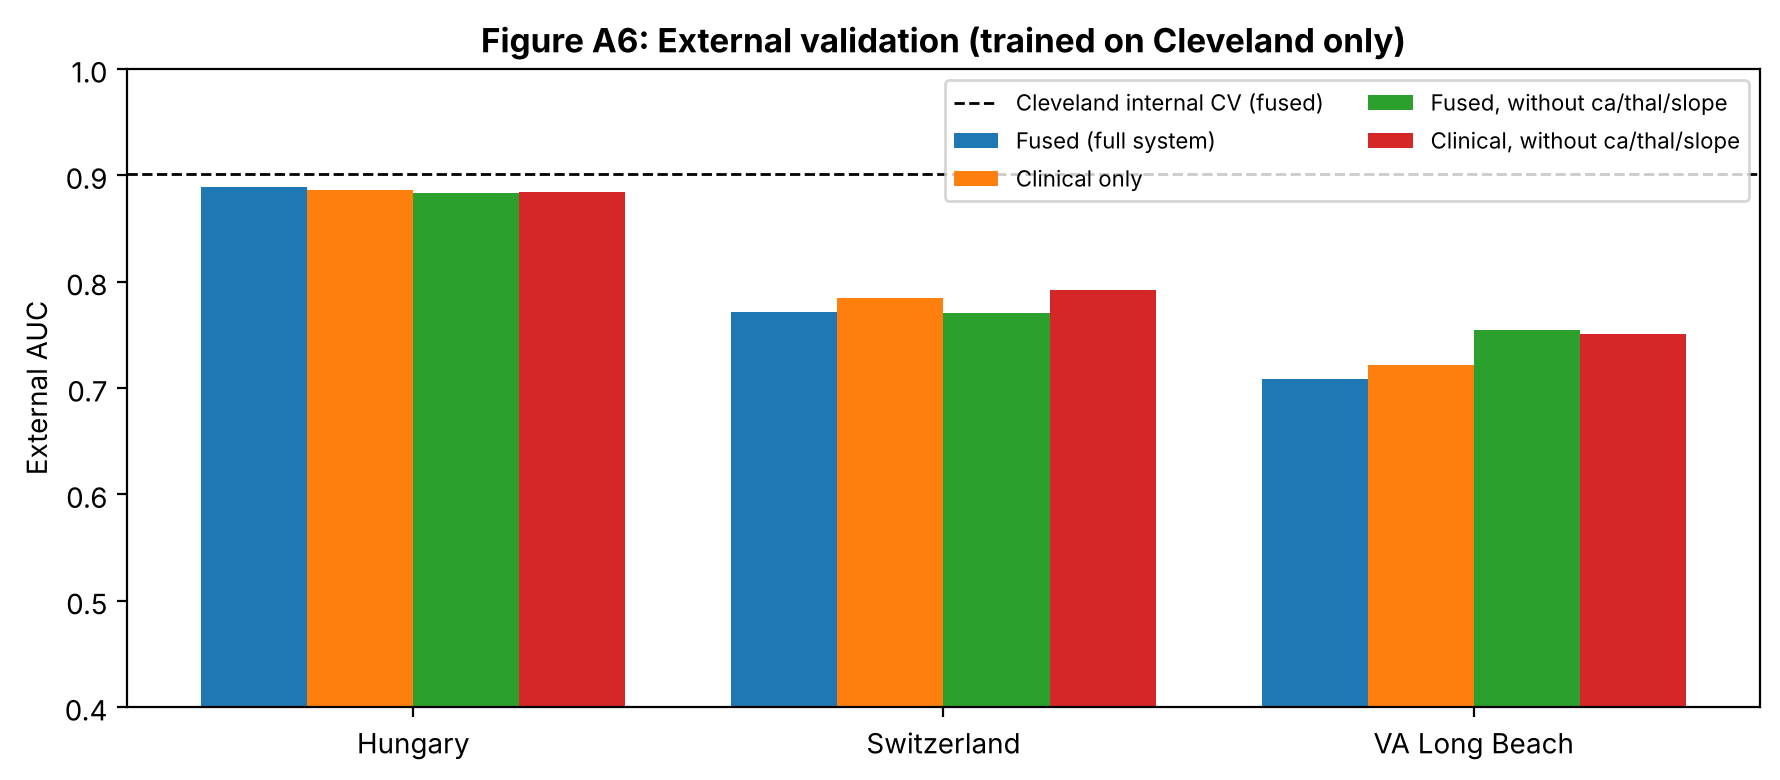
\includegraphics[width=\linewidth]{figA6_external.png}
\caption{External AUC of models trained on Cleveland only (dashed: Cleveland internal CV).}
\label{fig:a6}
\end{figure}

\subsection{SHAP Stability (RQ4)}
Attribution stability across 50 folds and 10 seeds, and agreement with permutation importance, are reported with the interpretation results in Section~VII (Tables~\ref{tab:e8} and~\ref{tab:shaptop}).

\subsection{Cross-Attention in the Dual-Branch Network}
Table~\ref{tab:e9} compares six networks trained with identical preprocessing, SMOTE and training budget. The numerical check confirms the derivation of Section~IV-C: with sequence length 1 every attention weight equals 1.000000, and replacing the ECG query with random values leaves the output unchanged. Consistent with this, the v4 architecture (AUC \xattnAUC{}) performs like its linear equivalent (\linearAUC{}) and like plain concatenation (\concatAUC{}; $\Delta$ \dConcat{}). A token-level variant, in which each ECG-proxy feature attends over the 13 clinical features so that attention can actually weight them, reaches \tokensAUC{} ($\Delta$ \dTokens{}). The token-level variant only reaches the level of the clinical-only MLP (\mlpClinAUC{}); no network exceeds it, and all remain below the soft-voting ensemble (\fullAUC{}). Adding the proxy block to an MLP actually lowers AUC (single MLP on all 36 features), as expected when 303 patients are spread over more inputs. We therefore remove cross-attention from the proposed system and report the dual-branch network only as an ablation.

\input{generated/tab_e9.tex}

\subsection{PTB-XL ECG Branch}
The parallel ECG benchmark (D2; PTB-XL normal versus abnormal) was ablated in the same way (Table~\ref{tab:e10}). Lead~II with Efficient tsfresh features reaches AUC \ecgRefAUC{}. The choice of lead matters: V5 performs as well as Lead~II (\ecgVFiveAUC{}), while Lead~I (\ecgLeadIAUC{}) and V1 (\ecgVOneAUC{}) are weaker. The rich feature set is essential: the 10 Minimal statistics of Lead~II reach only \ecgMinIIAUC{} (significant drop), and 10 Minimal statistics from each of the 12 leads reach \ecgTwelveMinAUC{}. Adding the 12-lead statistics to the Lead-II descriptors gives \ecgTwelvePlusAUC{}, a small, non-significant gain, so with handcrafted statistics and $N=303$ most of the accessible information is already in one well-chosen lead. Fitting VarianceThreshold and scaling on all records, as in v4, has no measurable effect, and neither SMOTE nor the random forest of v4 improves on the reference. Increasing the training set to 1{,}212 records does not raise AUC appreciably (Table~\ref{tab:e10size}; \ecgSizeList{}), although accuracy and the precision of the estimate improve. Substantial gains from raw ECGs are known to require learned representations and far larger datasets~\cite{ribeiro2020}. Signal quality matters: records with PTB-XL noise or electrode annotations ($n=\ecgNoisyN{}$) are classified with AUC \ecgNoisyAUC{} versus \ecgCleanAUC{} for clean records.

\input{generated/tab_e10.tex}
\input{generated/tab_e10size.tex}

\begin{figure}[!t]
\centering
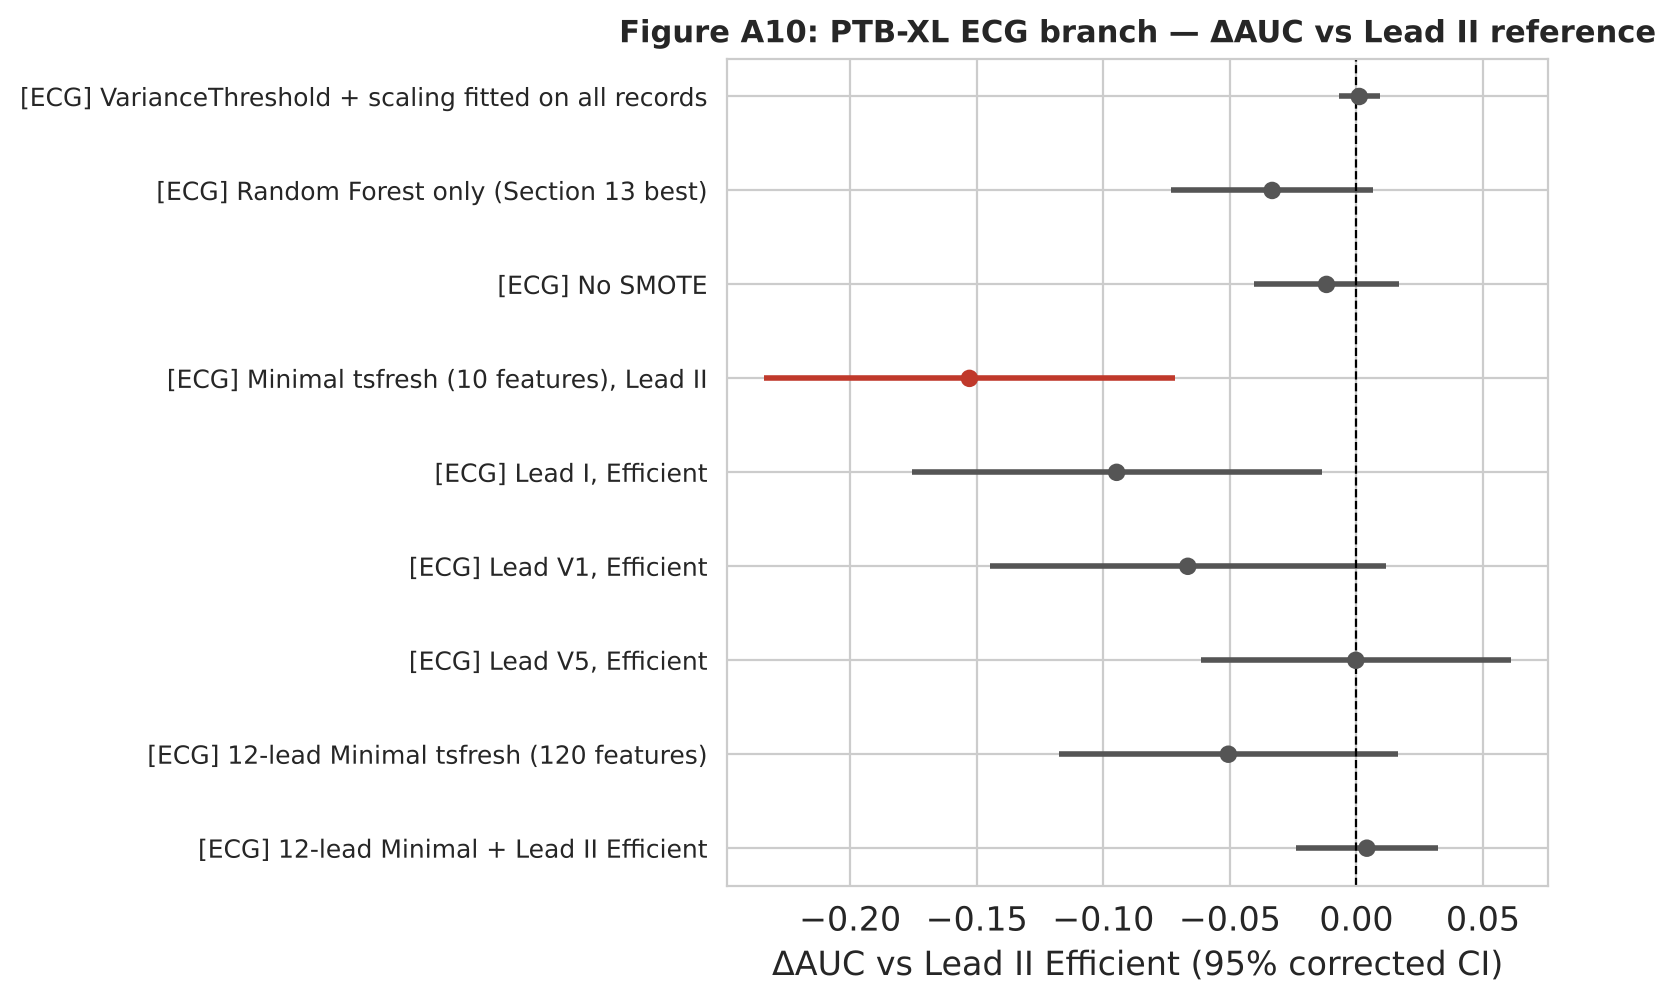
\includegraphics[width=\linewidth]{figA10_ptbxl_branch.png}
\caption{PTB-XL ECG-branch ablation: $\Delta$AUC versus Lead~II with Efficient tsfresh features.}
\label{fig:a10}
\end{figure}

\subsection{Summary: Which Claims Survive?}
Table~\ref{tab:verdict} re-tests each quantitative claim of the v4 manuscript.

\input{generated/tab_verdict.tex}



\section{Interpretability (RQ4)}
SHAP values describe how the fitted model uses its inputs. They are associational, not causal, and agreement with clinical knowledge is necessary but not sufficient evidence of validity (Section~II-D). We therefore report the explanations together with their stability, and we propose review by cardiologists as the appropriate next validation step.

\subsection{Global Feature Ranking}
Fig.~\ref{fig:shapglobal} (v4) shows the global TreeSHAP ranking of the XGBoost member on the seed-42 hold-out. Thallium scan result (\texttt{thal}), number of fluoroscopy-visible vessels (\texttt{ca}), chest-pain type (\texttt{cp}) and ST depression (\texttt{oldpeak}) dominate. This is consistent with clinical knowledge: a perfusion defect on thallium scintigraphy indicates ischaemia or scar, and vessels visualised on fluoroscopy reflect the coronary anatomy that the angiographic label describes. It also needs to be read with care. \texttt{ca} (vessels coloured by fluoroscopy) and \texttt{thal} (thallium stress scintigraphy) are results of advanced diagnostic tests carried out during the same diagnostic work-up that produced the angiographic label. A model that relies on them is a \emph{post-test} classifier, not a screening tool for patients who have not yet had these tests.

\begin{figure}[!t]
\centering
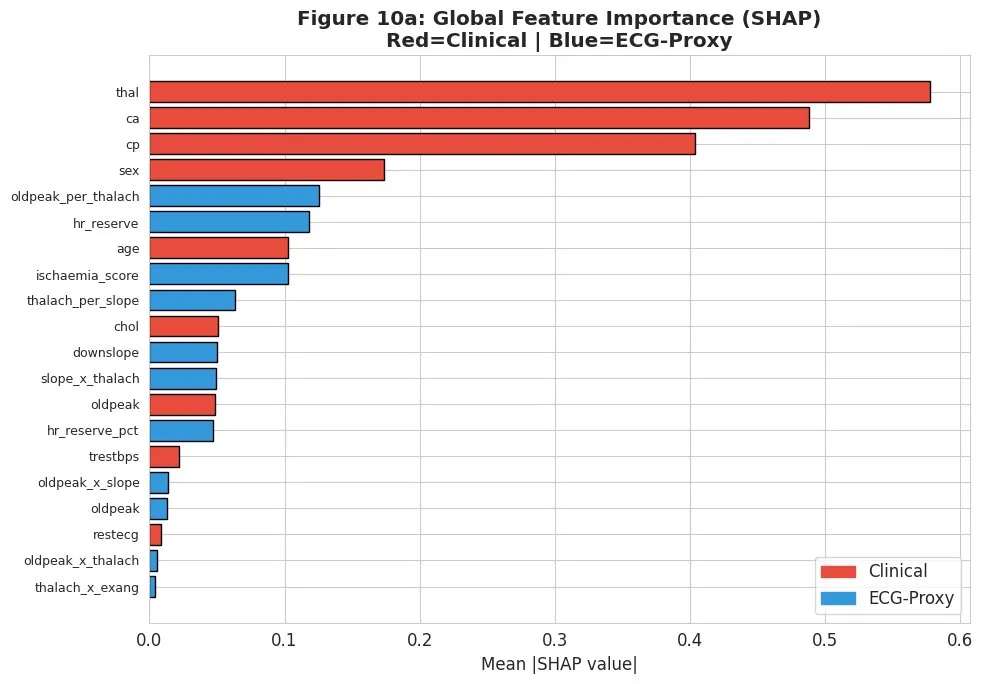
\includegraphics[width=0.92\linewidth]{fig4_shap_global.png}
\caption{Global SHAP importance of the XGBoost member on the v4 hold-out (red = clinical, blue = ECG-proxy).}
\label{fig:shapglobal}
\end{figure}

\subsection{Stability of the Ranking}
Repeating TreeSHAP in each of the 50 CV folds (Table~\ref{tab:e8}, Table~\ref{tab:shaptop}, Fig.~\ref{fig:a7}) shows that the \emph{top} of the ranking is stable while the tail is not. The fold-to-fold Spearman correlation of all 36 feature ranks is \shapRhoFold{}, and the top-5 sets overlap with a mean Jaccard index of \shapJac{}. Across ten training seeds on the full data the ranking correlation is \shapRhoSeed{}. Agreement with permutation importance on the same test folds is lower (Spearman \shapRhoPI{}). This is expected for correlated features: SHAP shares credit among correlated features, whereas permuting one of them leaves the information available through the others.

Under repeated CV, \texttt{cp}, \texttt{ca} and \texttt{thal} are in the top five in every fold (Table~\ref{tab:shaptop}). The ECG-proxy block nevertheless receives about a quarter of the total $|$SHAP$|$ mass, although removing it does not change AUC (Section~VI-A). The clearest case is \texttt{ischaemia\_score}, a product of \texttt{oldpeak}, \texttt{slope} and \texttt{exang}. It ranks fourth by mean $|$SHAP$|$ but its permutation importance is close to zero, and the raw \texttt{oldpeak} column itself falls far down the ranking because its derived terms absorb the credit. The duplicated columns show the same effect: \texttt{oldpeak}, \texttt{thalach}, \texttt{slope}, \texttt{exang} and \texttt{restecg} each appear twice in D3 and their attribution is split between identical copies (on average \dupShareMean{} goes to the proxy copy). The apparent importance of ``ECG-proxy'' features in Fig.~\ref{fig:shapglobal} is therefore \emph{redistributed} importance of the clinical exercise-test variables, not new information. SHAP rankings on engineered features should not be read as evidence that the engineering adds predictive value.

\begin{table}[!t]
\centering
\scriptsize
\caption{Stability of TreeSHAP attributions (XGBoost member) across 50 CV folds and 10 seeds.}
\label{tab:e8}
\setlength{\tabcolsep}{3pt}
\begin{adjustbox}{max width=\linewidth}
\begin{tabular}{lc}
\toprule
Stability measure & Mean (2.5--97.5\%) \\
\midrule
Spearman $\rho$ of SHAP rankings, fold vs fold (all 36 features) & 0.898 (2.5--97.5\%: 0.808--0.953) \\
Jaccard overlap of top-5 SHAP features, fold vs fold & 0.742 (2.5--97.5\%: 0.429--1.000) \\
Spearman $\rho$ of SHAP rankings, seed vs seed (full data) & 0.949 (2.5--97.5\%: 0.925--0.976) \\
Spearman $\rho$, SHAP vs permutation importance (same fold) & 0.270 (2.5--97.5\%: -0.273--0.761) \\
\bottomrule
\end{tabular}
\end{adjustbox}
\end{table}

\begin{table}[!t]
\centering
\scriptsize
\caption{Top-10 features by mean $|$SHAP$|$ over 50 folds, with rank stability and permutation importance (AUC drop).}
\label{tab:shaptop}
\setlength{\tabcolsep}{3pt}
\begin{adjustbox}{max width=\linewidth}
\begin{tabular}{llcccc}
\toprule
Feature & Block & Mean $|$SHAP$|$ & Median rank (IQR) & Top-5 & Perm.\ imp. \\
\midrule
cp & clinical & 0.515 & 2 (1--2) & 100\% & 0.0344 \\
ca & clinical & 0.498 & 2 (1--3) & 100\% & 0.0524 \\
thal & clinical & 0.453 & 3 (2--3) & 100\% & 0.0354 \\
ischaemia\_score & ECG-proxy & 0.162 & 4 (4--5) & 92\% & 0.0037 \\
sex & clinical & 0.119 & 6 (5--7) & 50\% & 0.0101 \\
age & clinical & 0.098 & 7 (5--8) & 28\% & 0.0043 \\
oldpeak\_per\_thalach & ECG-proxy & 0.093 & 7 (6--8) & 22\% & 0.0043 \\
hr\_reserve & ECG-proxy & 0.065 & 9 (8--11) & 2\% & 0.0002 \\
thalach\_per\_slope & ECG-proxy & 0.054 & 11 (9--14) & 2\% & -0.0018 \\
hr\_reserve\_pct & ECG-proxy & 0.052 & 11 (9--13) & 0\% & -0.0007 \\
\bottomrule
\end{tabular}
\end{adjustbox}
\end{table}


\begin{figure}[!t]
\centering
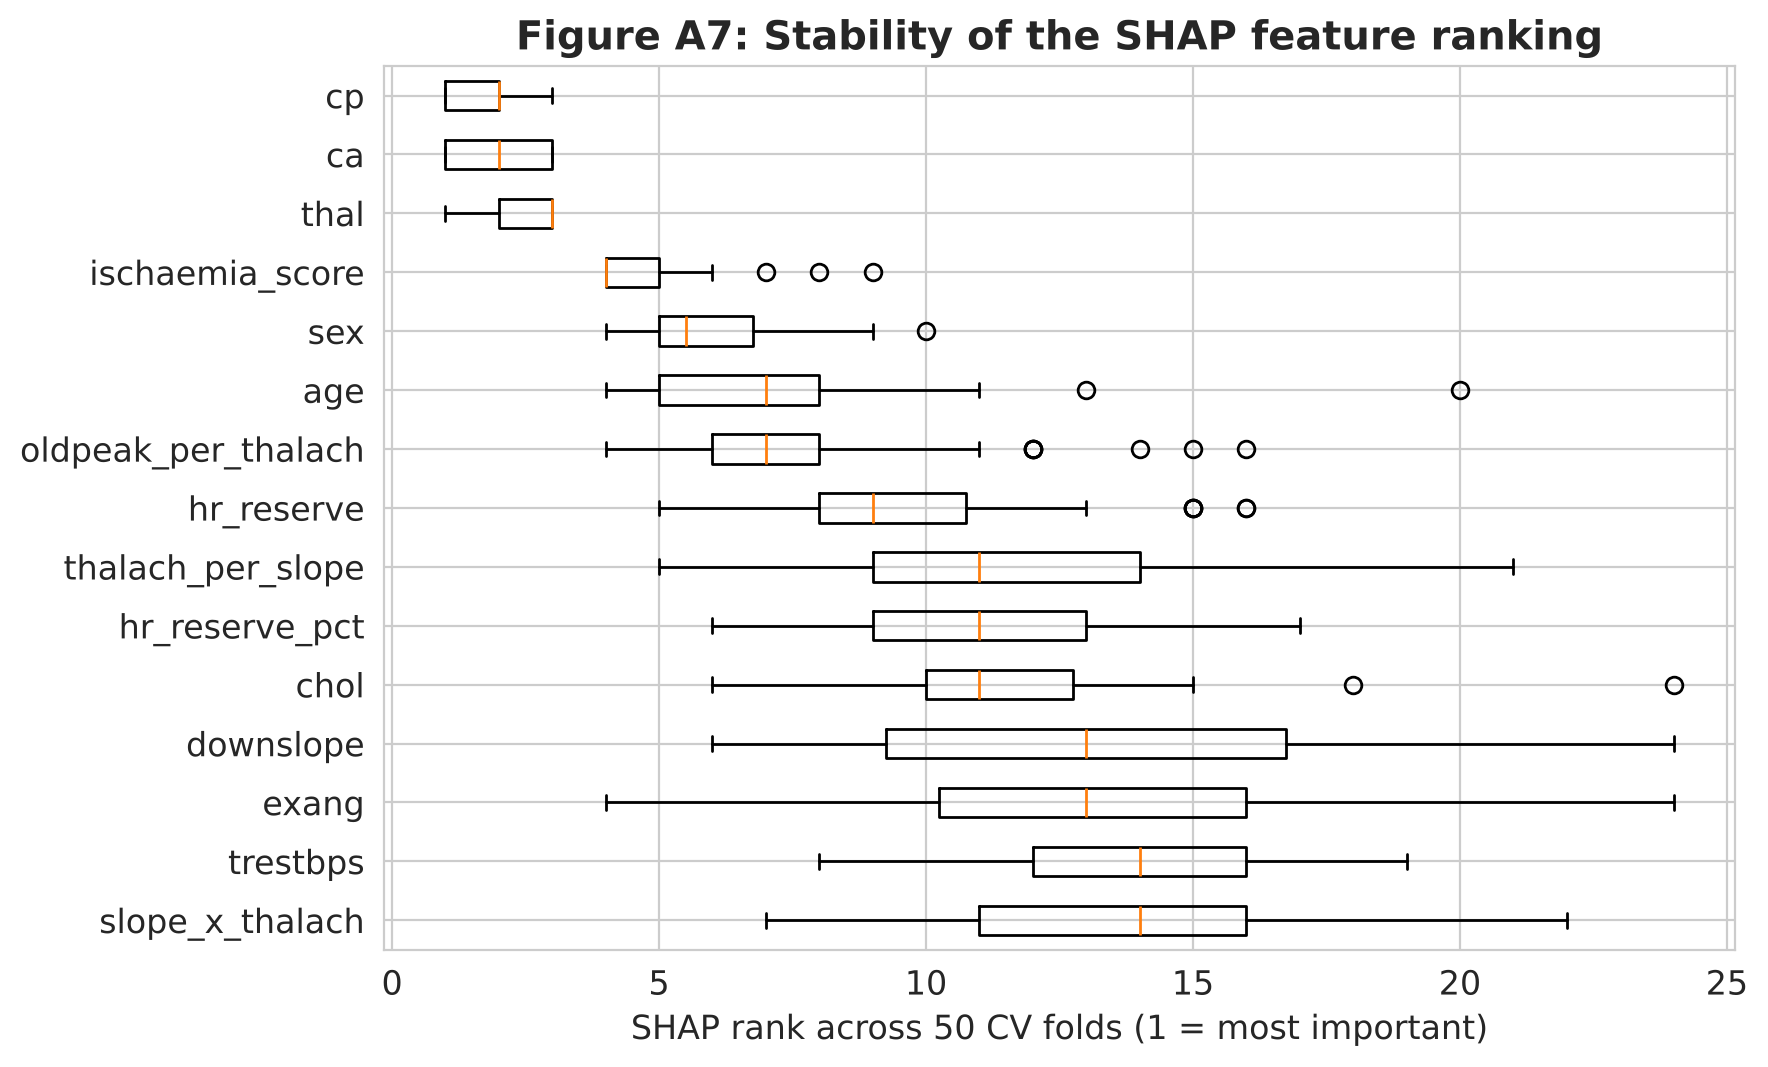
\includegraphics[width=\linewidth]{figA7_shap_rank_stability.png}
\caption{Distribution of each feature's SHAP rank across 50 CV folds.}
\label{fig:a7}
\end{figure}

\subsection{Dependence and Local Explanations}
Dependence plots (Fig.~\ref{fig:a8}) show directions consistent with clinical expectations. Risk rises with ST depression (\texttt{oldpeak}) and falls with higher maximal heart rate. It is higher for both fixed (6) and reversible (7) thallium defects than for a normal scan (3), and higher for asymptomatic chest pain (cp $=4$) than for the three symptomatic types. For \texttt{ca} the effect is essentially a step between 0 and $\geq$1 vessels, with little further increase for 2 or 3 vessels. The higher risk with asymptomatic chest pain reflects the referral population of this cohort, in which 73\% of patients without chest pain had CAD. It should not be read as a general clinical rule. Fig.~\ref{fig:a9} shows local explanations for one true-positive, false-negative, false-positive and true-negative patient. The false negative is a CAD patient whose chest-pain type, vessel count and thallium result all look benign (all three push the prediction towards ``healthy''); this failure mode cannot be fixed by ECG-proxy features derived from the same exercise test. The v4 interaction heatmap (Fig.~\ref{fig:heatmap}) is retained. Its clusters (oldpeak with its derived terms; thalach with slope products) arise largely because these features are functions of each other.

\begin{figure*}[!t]
\centering
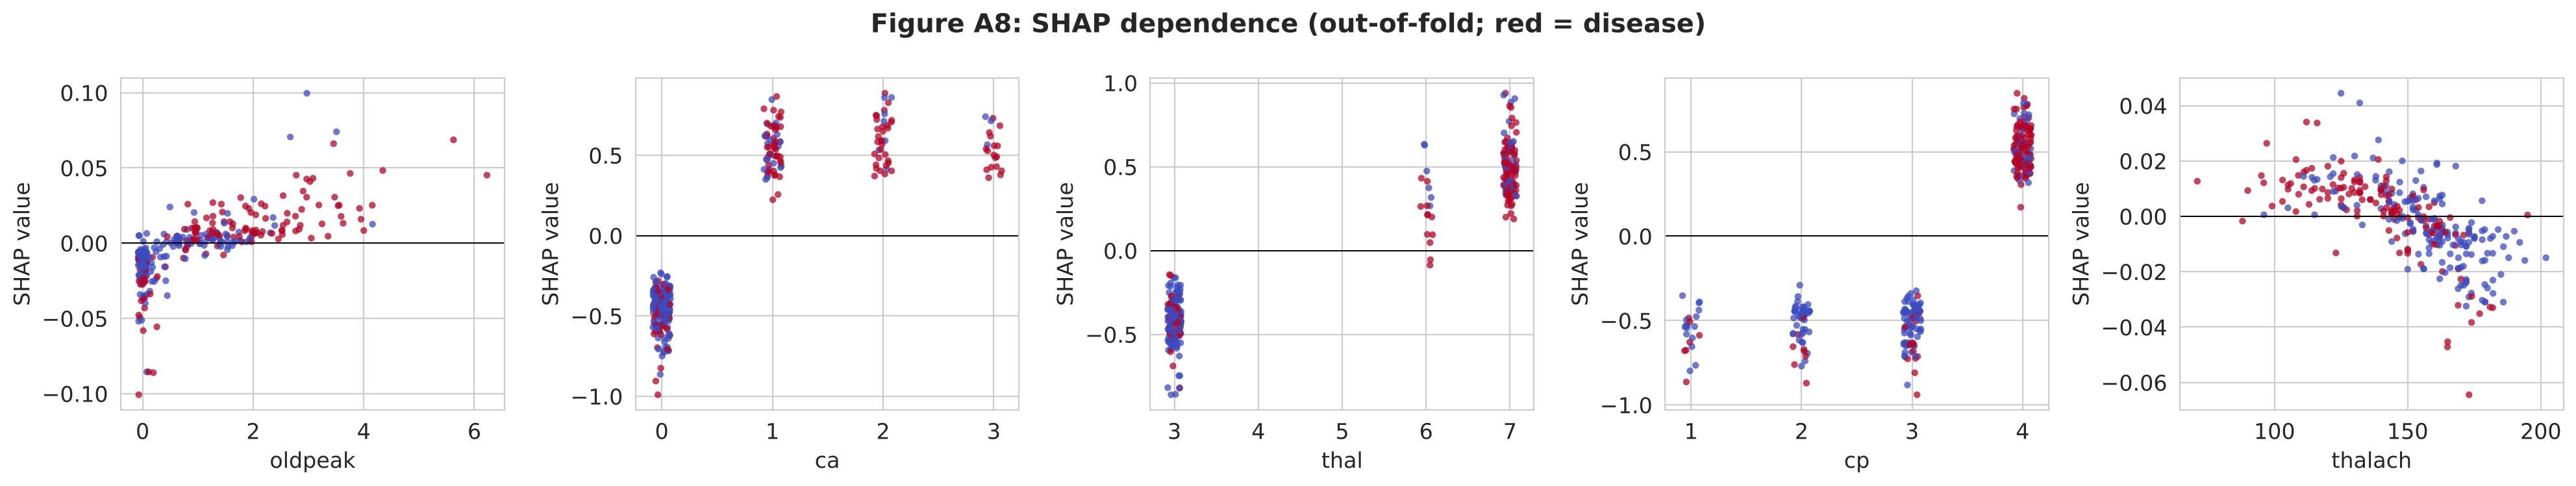
\includegraphics[width=\linewidth]{figA8_shap_dependence.png}
\caption{SHAP dependence for oldpeak, ca, thal, cp and thalach (out-of-fold, repeat 1; red = CAD).}
\label{fig:a8}
\end{figure*}

\begin{figure*}[!t]
\centering
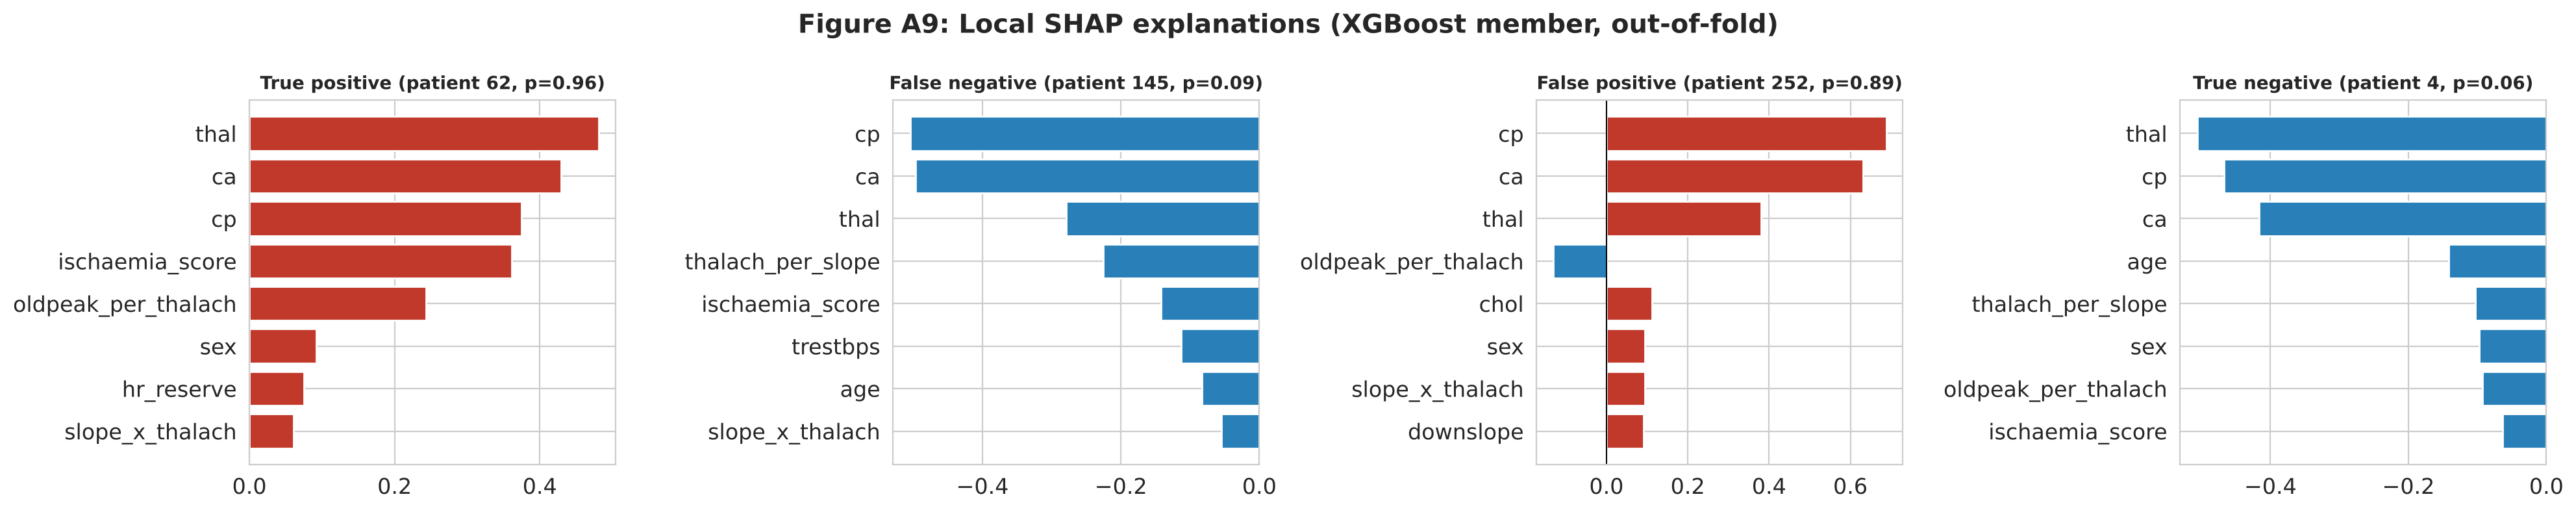
\includegraphics[width=\linewidth]{figA9_shap_local.png}
\caption{Local SHAP explanations (top-8 contributions) for one TP, FN, FP and TN patient.}
\label{fig:a9}
\end{figure*}

\begin{figure}[!t]
\centering
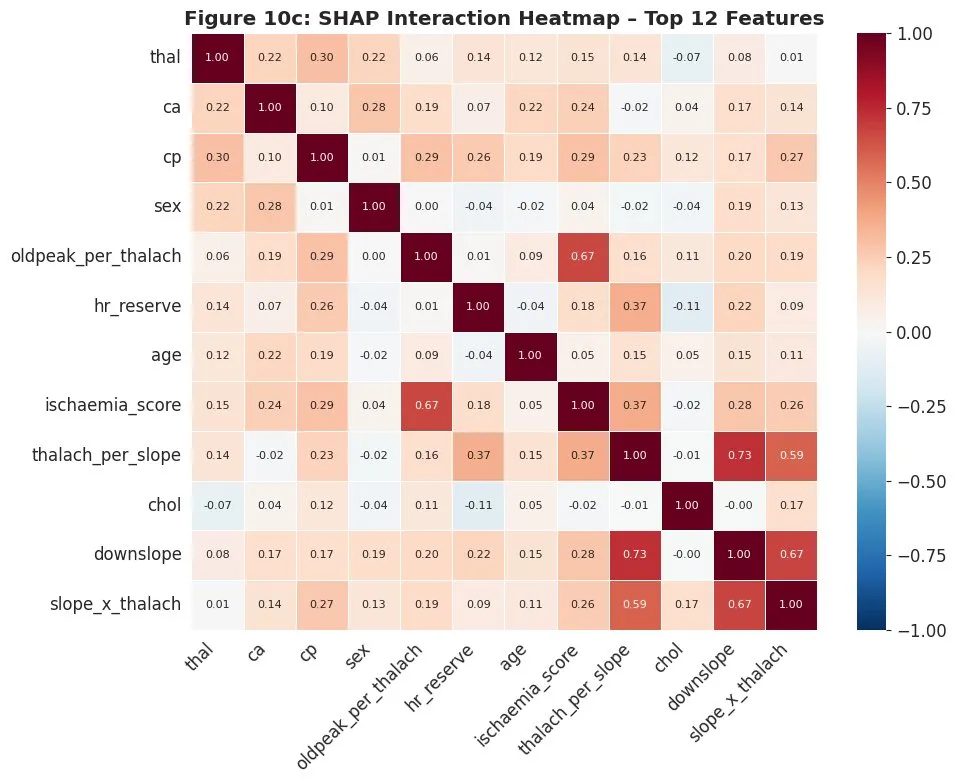
\includegraphics[width=0.9\linewidth]{fig5_shap_heatmap.png}
\caption{Correlation of SHAP values among the top-12 features (v4).}
\label{fig:heatmap}
\end{figure}

\section{Discussion}
\subsection{Protocol-Aware Comparison with Prior Work}
Under a leak-free, repeated-CV protocol the full system reaches AUC \fullAUC{} and accuracy \fullAcc{} on Cleveland. That is below the 89--99\% accuracies in Table~\ref{tab:lit} and below our own v4 hold-out figure. The gap is mostly methodological rather than a weakness of the model. Section~VI-D shows that a favourable single split can add about 7 points of accuracy, and oversampling before CV inflates AUC. Published Cleveland results should be compared only when their protocols are known to be equivalent, and we recommend that future work report repeated-CV estimates with corrected CIs, as done here.

\subsection{Why the ECG-Proxy Block Adds Nothing, and What the Model Learns}
The proxy features are deterministic functions of five clinical columns that the classifiers already see. Tree ensembles can represent products, ratios and thresholds through successive splits, and an RBF-SVM through its kernel, so the engineered terms add redundancy but no information. The control experiments (Section~VI-B) confirm that the block behaves like any other set of redundant columns. Predictive signal comes mainly from \texttt{cp}, \texttt{ca} and \texttt{thal}. Two of these, vessel count by fluoroscopy and thallium scintigraphy, come from the same invasive or nuclear work-up that produces the angiographic label, so the model is best described as a \emph{post-test} classifier rather than a screening tool. Without them, AUC falls to \robRestFu{} on resting data alone (Section~VI-E), and external sites, where these tests are mostly missing, show lower discrimination (Section~VI-G). The clinically useful contributions of this pipeline are therefore its calibrated, explainable risk estimates and the quantification of which tests drive them, not a fusion gain.

\subsection{Non-Significant Results}
The v4 manuscript reported non-significant tests ($p=1.00$, $p=0.72$) but still described the fusion benefit as ``practically meaningful''. The present results show that this interpretation is not justified. The paired clinical$-$fused AUC difference is \dClinAUC{}. Its CI is centred near zero, and its lower bound excludes any fusion gain larger than about 0.01 AUC, so the study is not merely underpowered. With 50 paired folds it can rule out the large effects claimed in v4. Absence of evidence for a small gain remains possible; detecting a gain of $\leq$0.01 AUC would require several thousand patients~\cite{vabalas2019}.

\subsection{Answers to the Research Questions}
\textbf{RQ1} (proxy features): No. $\Delta$AUC \dClinAUC{} in favour of clinical-only, no feature group matters, and noise controls perform equally well.
\textbf{RQ2} (components): Probabilistic ensembling matters (hard voting $-$0.03 AUC; single RF or GBM $-$0.02), but soft voting is no better than SVM or logistic regression alone. SMOTE and the choice of imbalance strategy do not matter on this mildly imbalanced dataset. Cross-attention adds nothing (Section~VI-I).
\textbf{RQ3} (robustness): Conclusions are unchanged under 16 perturbations, across subgroups and at three external sites. Generalisation is limited mainly by missing \texttt{ca}/\texttt{thal} rather than by the feature set. Hold-out estimates from a single split are unreliable.
\textbf{RQ4} (explanations): The top of the SHAP ranking (\texttt{cp}, \texttt{ca}, \texttt{thal}) is stable across folds and seeds. Credit assigned to engineered features is redistributed from their parent variables and does not indicate added value.

\subsection{Limitations}
\emph{Cohort size and setting.} Cleveland has 303 patients from one centre, collected in the 1980s, with a referral population. External validation was possible only on three historical cohorts with heavy missingness, and no cohort of South Asian, Sub-Saharan African or East Asian patients was available.
\emph{No paired ECG data.} Cleveland and PTB-XL contain different patients, so true clinical--ECG fusion could not be evaluated. The proxy features approximate ECG information from five exercise-test variables, and PTB-XL serves only as a parallel benchmark with a different label construct.
\emph{Single lead and statistical descriptors.} The main ECG branch uses Lead~II and tsfresh statistics rather than clinical ECG biomarkers (QTc, PR, QRS duration); Section~VI-J quantifies part of this.
\emph{Hyper-parameters} were tuned once on the v4 training split. Nested tuning gave similar results for XGBoost but was not repeated for every member.
\emph{Explanations} were not reviewed by clinicians.

\subsection{Future Work}
The most valuable next step is a cohort with paired clinical variables and raw ECGs for the same patients (e.g.\ MIMIC-IV-ECG with linked records), which would allow true fusion to be tested with the protocol developed here. Replacing tsfresh descriptors with representations from self-supervised ECG encoders, extending to 12 leads, multi-site or federated training, predicting stenosis severity (\texttt{num}~0--4), and a structured clinician review of the SHAP explanations are further directions.

\section{Conclusion}
This revision re-examined MultiCardioFusion, an explainable pipeline that enriches the 13 Cleveland clinical variables with 23 ECG-proxy features and benchmarks a parallel PTB-XL ECG branch, under a controlled ablation protocol of \nVariants{} configurations. The system discriminates CAD well (AUC \fullAUC{} \fullAUCci{} under leak-free repeated CV; up to \extHunFu{} at an external hospital) and its explanations are stable for the dominant predictors. The central v4 claim, however, does not survive: the ECG-proxy block does not improve on the clinical variables alone ($\Delta$AUC \dClinAUC{} in favour of clinical-only). It behaves like added noise in control experiments, does not help under 16 perturbations, in any subgroup or at any external site, and the reported $+7.04$~pp gain arose from comparing a favourable hold-out split (95th percentile of \hoN{} splits) with a cross-validation estimate. SMOTE, the specific imbalance strategy and cross-attention over a length-1 sequence likewise add nothing measurable, while the availability of \texttt{ca} and \texttt{thal}, and recalibration of the predicted probabilities, matter.

The contribution of this work is therefore a reproducible, leakage-aware and fully ablated baseline for explainable CAD prediction on Cleveland, together with a demonstration of how single-split evaluation, pre-CV oversampling and attribution to engineered features can produce misleading conclusions on small clinical datasets. Testing true clinical--ECG fusion requires a cohort in which both modalities come from the same patients; the protocol and code released with this paper are designed to be applied to such data directly.

\begin{thebibliography}{99}
\footnotesize
\bibitem{detrano1989} R.~Detrano \emph{et al.}, ``International application of a new probability algorithm for the diagnosis of coronary artery disease,'' \emph{Am. J. Cardiol.}, vol.~64, no.~5, pp.~304--310, 1989.
\bibitem{arabasadi2017} Z.~Arabasadi \emph{et al.}, ``Computer aided decision making for heart disease detection using hybrid neural network-genetic algorithm,'' \emph{Comput. Methods Programs Biomed.}, vol.~141, pp.~19--26, 2017.
\bibitem{haq2018} A.~U. Haq \emph{et al.}, ``A hybrid intelligent system framework for the prediction of heart disease using machine learning algorithms,'' \emph{Mobile Inf. Syst.}, vol.~2018, pp.~1--21, 2018.
\bibitem{mohan2019} S.~Mohan \emph{et al.}, ``Effective heart disease prediction using hybrid machine learning techniques,'' \emph{IEEE Access}, vol.~7, pp.~81542--81554, 2019.
\bibitem{khan2021} M.~A. Khan, ``An IoT framework for heart disease prediction based on MDCNN classifier,'' \emph{IEEE Access}, vol.~9, pp.~34717--34727, 2021.
\bibitem{wagner2020} P.~Wagner \emph{et al.}, ``PTB-XL, a large publicly available electrocardiography dataset,'' \emph{Sci. Data}, vol.~7, no.~1, p.~154, 2020.
\bibitem{latha2019} C.~B.~C. Latha and S.~C. Jeeva, ``Improving the accuracy of prediction of heart disease risk based on ensemble classification techniques,'' \emph{Inform. Med. Unlocked}, vol.~16, p.~100203, 2019.
\bibitem{gao2021} X.-Y. Gao \emph{et al.}, ``Improving the accuracy for analyzing heart diseases prediction based on the ensemble method,'' \emph{Complexity}, vol.~2021, p.~6663455, 2021.
\bibitem{hannun2019} A.~Y. Hannun \emph{et al.}, ``Cardiologist-level arrhythmia detection and classification in ambulatory electrocardiograms using a deep neural network,'' \emph{Nat. Med.}, vol.~25, no.~1, pp.~65--69, 2019.
\bibitem{christ2018} M.~Christ \emph{et al.}, ``Time series feature extraction on basis of scalable hypothesis tests (tsfresh),'' \emph{Neurocomputing}, vol.~307, pp.~72--77, 2018.
\bibitem{litjens2017} G.~Litjens \emph{et al.}, ``A survey on deep learning in medical image analysis,'' \emph{Med. Image Anal.}, vol.~42, pp.~60--88, 2017.
\bibitem{attia2019} Z.~I. Attia \emph{et al.}, ``Screening for cardiac contractile dysfunction using an artificial intelligence-enabled electrocardiogram,'' \emph{Nat. Med.}, vol.~25, no.~1, pp.~70--74, 2019.
\bibitem{zhang2022} X.~Zhang \emph{et al.}, ``Multi-view learning framework combining ECG and clinical data for cardiac diagnosis,'' \emph{IEEE J. Biomed. Health Inform.}, vol.~26, no.~3, pp.~1012--1020, 2022.
\bibitem{vaswani2017} A.~Vaswani \emph{et al.}, ``Attention is all you need,'' in \emph{Adv. Neural Inf. Process. Syst.}, 2017, pp.~5998--6008.
\bibitem{lundberg2017} S.~M. Lundberg and S.-I. Lee, ``A unified approach to interpreting model predictions,'' in \emph{Adv. Neural Inf. Process. Syst.}, 2017, pp.~4765--4774.
\bibitem{lundberg2018tree} S.~M. Lundberg \emph{et al.}, ``Consistent individualized feature attribution for tree ensembles,'' arXiv:1802.03888, 2018.
\bibitem{chawla2002} N.~V. Chawla \emph{et al.}, ``SMOTE: Synthetic minority over-sampling technique,'' \emph{J. Artif. Intell. Res.}, vol.~16, pp.~321--357, 2002.
\bibitem{alizadehsani2013} R.~Alizadehsani \emph{et al.}, ``A data mining approach for diagnosis of coronary artery disease,'' \emph{Comput. Methods Programs Biomed.}, vol.~111, no.~1, pp.~52--61, 2013.
\bibitem{lyu2020} Q.~Lyu \emph{et al.}, ``Multi-label cardiac arrhythmia classification from electrocardiogram with deep learning,'' in \emph{Proc. ICASSP}, 2020, pp.~1104--1108.
\bibitem{sharma2020} H.~Sharma and N.~Rizvi, ``Prediction of heart disease using machine learning algorithms,'' \emph{Int. J. Inf. Technol.}, vol.~12, no.~2, pp.~355--363, 2020.
\bibitem{pouriyeh2017} S.~Pouriyeh \emph{et al.}, ``A comprehensive investigation and comparison of machine learning techniques in the domain of heart disease classification,'' in \emph{Proc. IEEE ISCC}, 2017, pp.~204--207.
\bibitem{ribeiro2020} A.~H. Ribeiro \emph{et al.}, ``Automatic diagnosis of the 12-lead ECG using a deep neural network,'' \emph{Nat. Commun.}, vol.~11, no.~1, p.~1760, 2020.
\bibitem{lundberg2018sepsis} S.~M. Lundberg \emph{et al.}, ``Explainable machine-learning predictions for the prevention of hypoxaemia during surgery,'' \emph{Nat. Biomed. Eng.}, vol.~2, no.~10, pp.~749--760, 2018.
\bibitem{bi2021} W.~Bi \emph{et al.}, ``Application of support vector machine and unsupervised learning for detecting COVID-19 severity using cardiac MRI-derived radiomics features,'' \emph{Diagnostics}, vol.~11, no.~3, p.~545, 2021.
\bibitem{benjamin2019} E.~J. Benjamin \emph{et al.}, ``Heart disease and stroke statistics -- 2019 update,'' \emph{Circulation}, vol.~139, no.~10, pp.~e56--e528, 2019.
\bibitem{tison2018} G.~H. Tison \emph{et al.}, ``Passive detection of atrial fibrillation using a commercially available smartwatch,'' \emph{JAMA Cardiol.}, vol.~3, no.~5, pp.~409--416, 2018.
\bibitem{rossi2021} R.~A. Rossi \emph{et al.}, ``Precision medicine in patients with heart failure,'' \emph{Heart Fail. Clin.}, vol.~17, no.~2, pp.~199--214, 2021.
\bibitem{chen2016} T.~Chen and C.~Guestrin, ``XGBoost: A scalable tree boosting system,'' in \emph{Proc. ACM SIGKDD}, 2016, pp.~785--794.
\bibitem{breiman2001} L.~Breiman, ``Random forests,'' \emph{Mach. Learn.}, vol.~45, no.~1, pp.~5--32, 2001.
\bibitem{cortes1995} C.~Cortes and V.~Vapnik, ``Support-vector networks,'' \emph{Mach. Learn.}, vol.~20, no.~3, pp.~273--297, 1995.
\bibitem{kingma2015} D.~P. Kingma and J.~Ba, ``Adam: A method for stochastic optimization,'' in \emph{Proc. ICLR}, 2015.
\bibitem{ioffe2015} S.~Ioffe and C.~Szegedy, ``Batch normalization,'' in \emph{Proc. ICML}, 2015, pp.~448--456.
\bibitem{srivastava2014} N.~Srivastava \emph{et al.}, ``Dropout: A simple way to prevent neural networks from overfitting,'' \emph{J. Mach. Learn. Res.}, vol.~15, no.~1, pp.~1929--1958, 2014.
\bibitem{pedregosa2011} F.~Pedregosa \emph{et al.}, ``Scikit-learn: Machine learning in Python,'' \emph{J. Mach. Learn. Res.}, vol.~12, pp.~2825--2830, 2011.
\bibitem{james2021} G.~James \emph{et al.}, \emph{An Introduction to Statistical Learning with Applications in R}, 2nd~ed. New York, NY, USA: Springer, 2021.
\bibitem{who2023} World Health Organization, ``Cardiovascular diseases (CVDs) -- key facts,'' WHO Fact Sheet, 2023. [Online]. Available: \url{https://www.who.int/news-room/fact-sheets/detail/cardiovascular-diseases-(cvds)}
\bibitem{hossain2023} M.~M. Hossain, M.~R. Islam, S.~A. Hossain, and M.~A. Moni, ``Heartbeat classification based on single Lead-II ECG using deep learning,'' \emph{Healthcare}, vol.~11, no.~15, p.~2183, 2023.
\bibitem{janosi1989} A.~Janosi, W.~Steinbrunn, M.~Pfisterer, and R.~Detrano, ``Heart Disease,'' UCI Machine Learning Repository, 1989. doi: 10.24432/C52P4X.
\bibitem{nadeau2003} C.~Nadeau and Y.~Bengio, ``Inference for the generalization error,'' \emph{Mach. Learn.}, vol.~52, no.~3, pp.~239--281, 2003.
\bibitem{bouckaert2004} R.~R. Bouckaert and E.~Frank, ``Evaluating the replicability of significance tests for comparing learning algorithms,'' in \emph{Proc. PAKDD}, 2004, pp.~3--12.
\bibitem{holm1979} S.~Holm, ``A simple sequentially rejective multiple test procedure,'' \emph{Scand. J. Statist.}, vol.~6, no.~2, pp.~65--70, 1979.
\bibitem{ojala2010} M.~Ojala and G.~C. Garriga, ``Permutation tests for studying classifier performance,'' \emph{J. Mach. Learn. Res.}, vol.~11, pp.~1833--1863, 2010.
\bibitem{vancalster2019} B.~Van~Calster \emph{et al.}, ``Calibration: the Achilles heel of predictive analytics,'' \emph{BMC Med.}, vol.~17, p.~230, 2019.
\bibitem{huang2020fusion} S.-C. Huang \emph{et al.}, ``Fusion of medical imaging and electronic health records using deep learning: a systematic review and implementation guidelines,'' \emph{npj Digit. Med.}, vol.~3, p.~136, 2020.
\bibitem{kumar2020problems} I.~E. Kumar \emph{et al.}, ``Problems with Shapley-value-based explanations as feature importance measures,'' in \emph{Proc. ICML}, 2020, pp.~5491--5500.
\bibitem{molnar2022pitfalls} C.~Molnar \emph{et al.}, ``General pitfalls of model-agnostic interpretation methods for machine learning models,'' in \emph{xxAI -- Beyond Explainable AI}, LNCS vol.~13200, Springer, 2022, pp.~39--68.
\bibitem{slack2020fooling} D.~Slack \emph{et al.}, ``Fooling LIME and SHAP: Adversarial attacks on post hoc explanation methods,'' in \emph{Proc. AAAI/ACM Conf. AI, Ethics, Society}, 2020, pp.~180--186.
\bibitem{he2008adasyn} H.~He \emph{et al.}, ``ADASYN: Adaptive synthetic sampling approach for imbalanced learning,'' in \emph{Proc. IEEE IJCNN}, 2008, pp.~1322--1328.
\bibitem{han2005borderline} H.~Han, W.-Y. Wang, and B.-H. Mao, ``Borderline-SMOTE: A new over-sampling method in imbalanced data sets learning,'' in \emph{Proc. ICIC}, 2005, pp.~878--887.
\bibitem{gorishniy2021} Y.~Gorishniy \emph{et al.}, ``Revisiting deep learning models for tabular data,'' in \emph{Adv. Neural Inf. Process. Syst.}, 2021, pp.~18932--18943.
\bibitem{vabalas2019} A.~Vabalas \emph{et al.}, ``Machine learning algorithm validation with a limited sample size,'' \emph{PLoS ONE}, vol.~14, no.~11, p.~e0224365, 2019.
\end{thebibliography}


\end{document}
